\documentclass[UTF8]{ctexart}
\usepackage{graphicx}
\usepackage{float}
\usepackage{fancyhdr}
\usepackage{listings}
\usepackage{xeCJK} 
\usepackage{authblk} 
\usepackage{geometry}
\usepackage{hyperref}
\usepackage{amsmath, amsthm, amssymb, amsfonts}
\usepackage{thmtools}
\usepackage{ctex}
\usepackage{graphicx}
\usepackage{setspace}
\usepackage{geometry}
\usepackage{float}
\usepackage{hyperref}
\usepackage[utf8]{inputenc}
\usepackage[english]{babel}
\usepackage{framed}
\usepackage[dvipsnames]{xcolor}
\usepackage{tcolorbox}
\usepackage{algorithm}
\usepackage{algorithmic}
\usepackage{tikz}
\usepackage{booktabs}
\usepackage{array}
\usepackage{multirow}
\usepackage{tabularx} % 用于设置表格宽度
\usepackage{xcolor}   % 用于表格中使用颜色
\usepackage{colortbl} % 用于彩色表格
%for long table
\usepackage{longtable}

%for table toprule line
\usepackage{booktabs}

\colorlet{LightGray}{White!90!Periwinkle}
\colorlet{LightOrange}{Orange!15}
\colorlet{LightGreen}{Green!15}
\bibliographystyle{plain}
\geometry{a4paper}
\geometry{left=2cm} 
\geometry{right=2cm} 
\geometry{top=3cm} 
\geometry{bottom=3cm} 
\pagestyle{fancy}
\fancyhf{}
\newcommand{\HRule}[1]{\rule{\linewidth}{#1}}
\usetikzlibrary{trees}
\definecolor{EE}{RGB}{147, 233, 192}
\definecolor{TT}{RGB}{112, 182, 151}
\definecolor{FF}{RGB}{75, 128, 107}
\definecolor{oo}{RGB}{35, 71, 60}
\declaretheoremstyle[name=Theorem,]{thmsty}
\declaretheorem[style=thmsty,numberwithin=section]{theorem}
\tcolorboxenvironment{theorem}{colback=LightGray}
\usetikzlibrary{shapes.geometric, arrows.meta, positioning,arrows,automata}
\tikzset{
    startstop/.style={rectangle, rounded corners, minimum width=3cm, minimum height=1cm, text centered, draw=black, fill=blue!30},
    process/.style={rectangle, minimum width=3cm, minimum height=1cm, text centered, draw=black, fill=blue!15},
    arrow/.style={thick, ->, >=stealth},
}

\setstretch{1.2}
\geometry{
    textheight=9in,
    textwidth=5.5in,
    top=1in,
    headheight=12pt,
    headsep=25pt,
    footskip=30pt
}

\lstset{
    numbers=left, 
    numberstyle= \tiny, 
    keywordstyle= \color{ blue!70},%设置关键字颜色
    commentstyle= \color{red!50!green!50!blue!50}, %设置注释颜色
    frame=shadowbox, % 阴影效果
    rulesepcolor= \color{ red!20!green!20!blue!20} ,
    escapeinside=``, % 英文分号中可写入中文
    xleftmargin=2em, %距离左边界2em
    aboveskip=1em,
    framexleftmargin=2em,
    basicstyle=\ttfamily,
    columns=fullflexible,%可以自动换行
    linewidth=1\linewidth, %设置代码块与行同宽
    breaklines=true,%在单词边界处换行。
    showstringspaces=false, %去掉空格时产生的下划的空格标志, 设置为true则出现
    breakatwhitespace=ture,%可以在空格处换行
    escapechar=`%设置转义字符为反引号
}
\rhead{Choimoe/SDUCompilerPrinciplesHomework}
\lhead{编译原理与技术课程作业}
\rfoot{\thepage}
\begin{document}
\title{ \normalsize \textsc{}
		\\ [2.0cm]
		\HRule{2.0pt} \\
		\LARGE \textbf{{编译原理与技术课程作业}
		\HRule{2.0pt} \\ [0.6cm] {————作业1\;\textasciitilde\;9\;合集} \vspace*{10\baselineskip}}
		}
\date{}
\author{Choimoe \\ 
		\href{https://github.com/Choimoe/SDUCompilerPrinciplesHomework}{https://github.com/Choimoe/SDUCompilerPrinciplesHomework} \\
		SDU 编译原理与技术课程作业 \\
		2024.12.31}

\maketitle

\newpage
\tableofcontents

\newpage
	% 代码分析:模块功能、涉及到的类、类关系、数据结构及关键代码等;
	% 任务要求,设计任务要求;
	% 设计:详细的设计方案,相关的数据结构、算法描述,可采用伪代码等形式化描述
	% 实现:修改哪些类、如何修改、为什么修改等;
	% 测试:测试用例,测试结果及结果分析,测试运行界面等;
	% 调试:调试方法,遇到的问题及解决方案等;
	% 结论与展望:完成的主要工作、收获、进一步的工作,建议、体会、心得等;

\section{作业1}
\subsection{作业1.1}
\subsubsection{题目描述}
画图表示编译过程的各个阶段,并简要说明各阶段的功能。

\subsubsection{解答}
\begin{figure}[H]
    \centering
    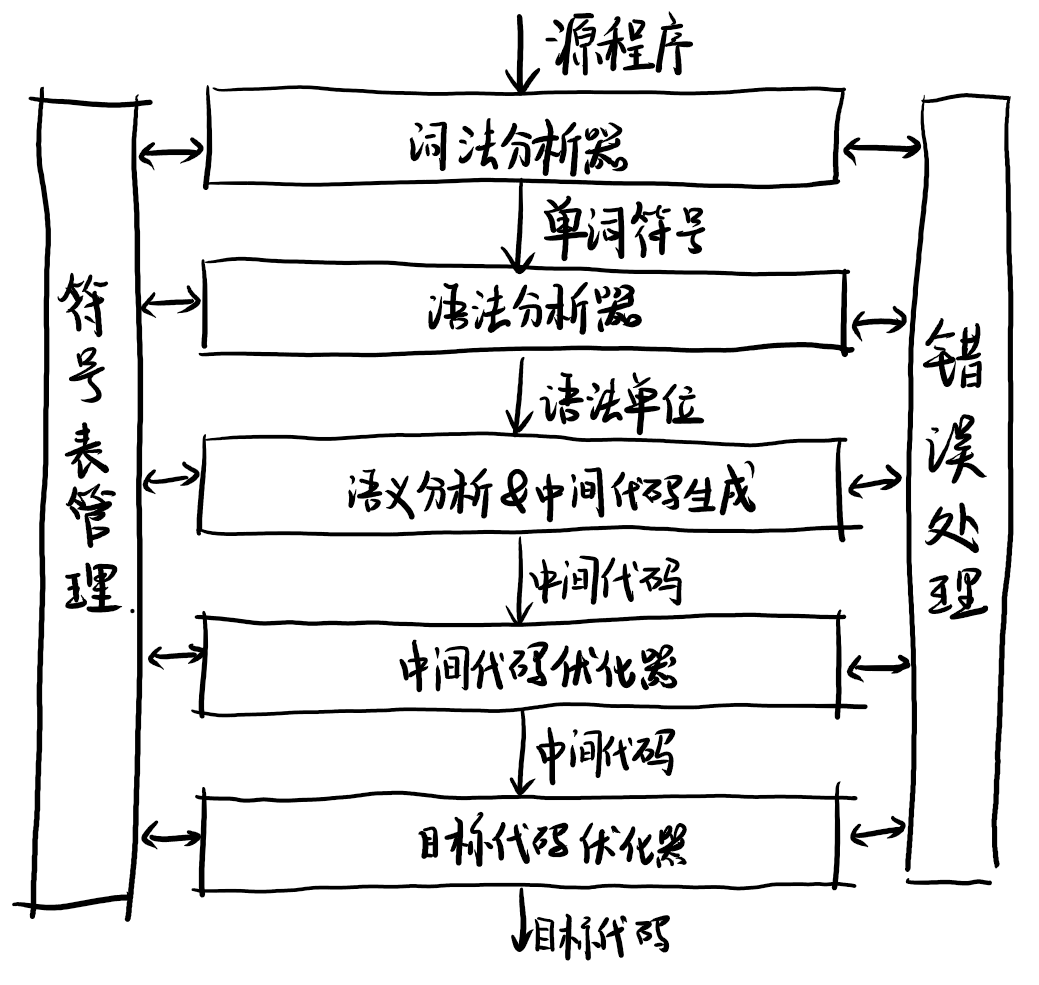
\includegraphics[width=0.6\linewidth]{imgs/编译过程.png}
    \caption{编译过程的阶段}
    \label{fig:编译过程阶段}
\end{figure}

\begin{enumerate}
\item \textbf{词法分析器}:又称扫描器,输入源程序,进行词法分析,输出单词符号。
\item \textbf{语法分析器}:又称扫描器,对单词符号串进行语法分析,识别出各类语法单位,最终判断输入串是否构成语法上正确的“程序”。
\item \textbf{语义分析与中间代码生成}:按照语义规则对语法分析器归约(或推导)出的语法单位进行语义分析,并把它们翻译成一定形式的中间代码。
\item \textbf{中间代码优化器}:对中间代码进行优化处理。
\item \textbf{目标代码生成器}:把中间代码翻译成目标代码。
\item \textbf{错误处理}:发现各种错误、准确指出错误的性质和发生错误的地点、将错误所造成的影响限制在尽可能小的范围、自动校正错误(如果可能)。
\item \textbf{符号表}:用于登记源程序的各类信息和编译各阶段的进展状况。
\end{enumerate}

\subsection{作业1.2}
\subsubsection{题目描述}
求表达式 “$a \vee b \neq c+d \land a * b<f$” 的后缀式。
\subsubsection{解答}
\begin{table}[h]
\centering
\begin{tabular}{>{\centering\arraybackslash}m{3cm}>{\centering\arraybackslash}m{3cm}>{\centering\arraybackslash}m{4cm}>{\centering\arraybackslash}m{3cm}}
\toprule
\textbf{类别} & \textbf{算符} & \textbf{符号} & \textbf{结合性} \\
\midrule
位运算符 & 按位取反 & $\sim$ & 右结合 \\
\midrule
\multirow{3}{*}{算术算符} & 幂、负 & $**, -(@)$ & 右结合 \\
\cmidrule{2-4}
 & 乘除、取余 & $* (\times), /(\div), \%$ & 左结合 \\
\cmidrule{2-4}
 & 加减 & $+, -$ & 左结合 \\
\midrule
位运算符 & 左移、右移 & $\ll, \gg$ & 左结合 \\
\midrule
\multirow{2}{*}{关系算符} & 大于小于 & $<,\leq, >,\geq$ & 不可结合 \\
\cmidrule{2-4}
 & 等于不等 & $=, \neq$ & 不可结合 \\
\midrule
\multirow{3}{*}{位运算符} & 按位与 & $\&$ & 左结合 \\
\cmidrule{2-4}
 & 按位异或 & $\oplus$ & 左结合 \\
\cmidrule{2-4}
 & 按位或 & $|$ & 左结合 \\
\midrule
\multirow{3}{*}{逻辑算符} & 非 & $\neg , !, \text{或 \textbf{not}}$ & 右结合 \\
\cmidrule{2-4}
 & 与 & $\land ,\&\&, \text{或 \textbf{and}}$ & 左结合 \\
\cmidrule{2-4}
 & 或 & $\lor ,||, \text{或 \textbf{or}}$ & 左结合 \\
\midrule
三目算符 & 三目算符 & $?$ : & 右结合 \\
\midrule
赋值算符 & 赋值等 & $= \text{或 :=}$ & 右结合 \\
\bottomrule
\end{tabular}
\end{table}
按照算符优先级,有:
\begin{align*}
& {\color{Red} <}  a \vee b \neq c+d \land a * b<f{\color{Red} >}  \\
= & {\color{Red} <}  a{\color{Red} >} {\color{Red} <} b \neq c+d \land a * b<f{\color{Red} >} \vee\\
= & a {\color{Red} <} b \neq c+d {\color{Red} >}{\color{Red} <} a * b<f{\color{Red} >}\land \vee\\
= & a{\color{Red} <} b{\color{Red} >} {\color{Red} <}c+d{\color{Red} >}\neq{\color{Red} <} a * b{\color{Red} >}{\color{Red} <}f{\color{Red} >}<\land \vee\\
= & abcd+\neq ab*f<\land \vee
\end{align*}


\subsection{作业1.3}
\subsubsection{题目描述}
编写汇编程序:
\begin{enumerate}
    \item 在静态数据区声明 3 个 32 位变量 a、b、c,其中 a、b 初始化为 10 和 20,c 不初始化;
    \item 在代码区编写代码,将 a + b 的结果保存到变量c。
\end{enumerate}
\subsubsection{解答}

使用在 1.3.6 传送指令 与 1.3.7 基本运算指令 中学到的指令:

\begin{lstlisting}[language={[x86masm]Assembler},title={指令集}]
add reg, imm/reg/mem ;两个操作数相加,结果存入第一个操作数的寄存器。
mov mem, imm/reg ;第一个操作数是目的操作数,第二个操作数是源操作数。
\end{lstlisting}

不难写出:

\begin{lstlisting}[language={[x86masm]Assembler},title={addition.s}]
section .data
    a dd 10
    b dd 20
    c dd 0
section .text
global _start
_start:
    mov eax, [a]
    add eax, [b]
    mov [c], eax
    mov eax, 1
    int 0x80
\end{lstlisting}

这里使用 sys\_exit 信号退出程序,可以使用 nasm 编译链接并执行:

\begin{lstlisting}[language=bash,title={bash}]
$ nasm -f elf64 -o addition.o addition.s
$ ld -o addition addition.o
$ ./addition
$ 
\end{lstlisting}

因为只有简单的相加所以没有输出,写输出程序有点麻烦,于是可以通过 gdb 来查看具体的值:

\begin{lstlisting}[language=bash,title={gdb}]
(gdb) break _start
Breakpoint 1 at 0x401000
(gdb) run
Starting program: /home/choimoe/Desktop/asm_learn/addition 
Breakpoint 1, 0x0000000000401000 in _start ()
(gdb) stepi
0x0000000000401007 in _start ()
(gdb) stepi
0x000000000040100e in _start ()
(gdb) p (int)c
$1 = 0
(gdb) stepi
0x0000000000401015 in _start ()
(gdb) p (int)c
$2 = 30
\end{lstlisting}



\newpage
\section{作业2}
\subsection{作业2.1}
\subsubsection{题目描述}

令文法为

\begin{align*}
E &\rightarrow E \vee T\;|\;T\\
T &\rightarrow T \wedge F\;|\; F\\
F &\rightarrow \neg F\;|\;(E)\;|\; i
\end{align*}

\begin{enumerate}
    \item 写出 $i \wedge(E)$  的最左推导和最右推导。
    \item 画出 $i_{1} \wedge \neg\left(i_{2} \vee i_{3}\right)$ 的语法树。
    \item 写出 $i_{1} \wedge \neg\left(i_{2} \vee i_{3}\right)$ 的所有短语、直接短语和句柄
\end{enumerate}

\subsubsection{解答}

\paragraph{题目 2.1.1} 若推导过程中,总是最先替换最右(左)的非终结符,则称为最右(左)推导:

\begin{align*}
E & \Rightarrow {\color{Green} T} \Rightarrow {\color{Green} T} \wedge F \Rightarrow {\color{Green} F}  \wedge F  \Rightarrow i \wedge {\color{Green} F}  \Rightarrow i \wedge (E) \\
E & \Rightarrow {\color{Green} T} \Rightarrow T \wedge {\color{Green} F} \Rightarrow {\color{Green} T}  \wedge (E) \Rightarrow {\color{Green} F}   \wedge (E) \Rightarrow i \wedge (E)
\end{align*}

\paragraph{题目 2.1.2} 首先写出一个推导:

\[
{\color{EE} E} \Rightarrow {\color{TT} T} \Rightarrow {\color{TT} T}{\color{oo} \wedge} {\color{FF} F} \Rightarrow {\color{FF} F}{\color{oo} \wedge\neg} {\color{FF} F} \Rightarrow {\color{oo}i_1}{\color{oo} \wedge\neg(}{\color{EE} E}{\color{oo} )} \Rightarrow {\color{oo}i_1}{\color{oo} \wedge\neg(}{\color{EE} E}\vee {\color{TT} T}{\color{oo} )} \overset {...} \Longrightarrow {\color{oo}i_1}{\color{oo} \wedge\neg (}{\color{oo}i_2} \vee {\color{oo}i_3}{\color{oo} )}
\]

于是可以画出语法树:

\begin{center} 
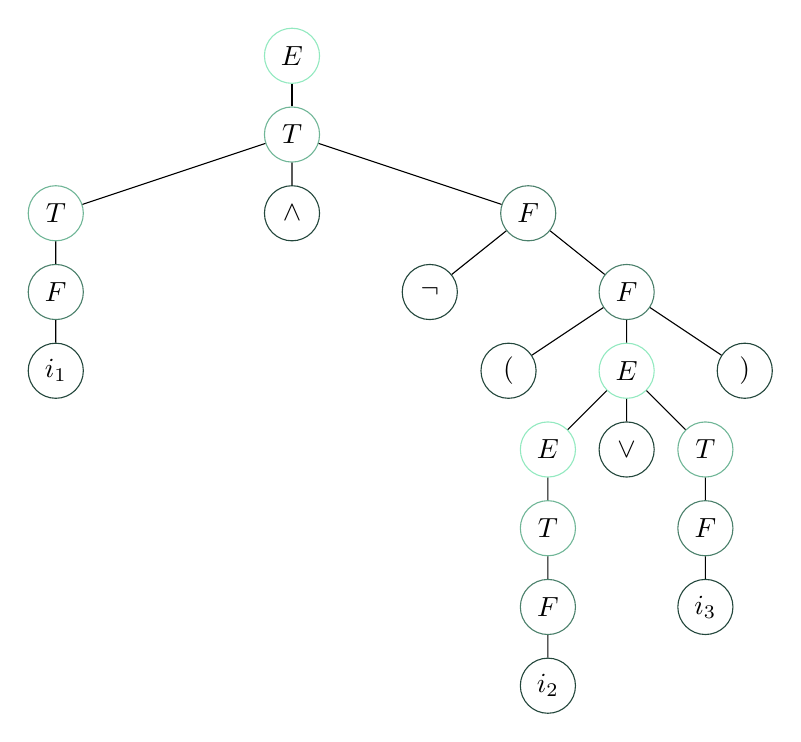
\begin{tikzpicture}[
  level distance=10mm, % 调整上下两行的间隔
  level 1/.style={sibling distance=40mm},
  level 2/.style={sibling distance=30mm},
  level 3/.style={sibling distance=25mm},
  level 4/.style={sibling distance=15mm},
  level 5/.style={sibling distance=10mm},
  every node/.style={draw, circle, minimum size=7mm, inner sep=2pt},
  colorE/.style={draw=EE},
  colorT/.style={draw=TT},
  colorF/.style={draw=FF},
  coloro/.style={draw=oo},
  ]

% Root node
\node[colorE]{$E$}
  child { node[colorT]{$T$}
    child { node[colorT]{$T$}
        child { node[colorF]{$F$}
            child { node[coloro]{$i_1$} }
        }
    }
    child { node[coloro]{$\wedge$} }
    child { node[colorF]{$F$} 
        child { node[coloro]{$\neg$} }
        child { node[colorF]{$F$}
            child { node[coloro]{$($} }
            child { node[colorE]{$E$}
                child { node[colorE]{$E$}
                    child { node[colorT]{$T$}
                        child { node[colorF]{$F$}
                            child { node[coloro]{$i_2$} }
                        }
                    }
                }
                child { node[coloro]{$\vee$} }
                child { node[colorT]{$T$}
                    child { node[colorF]{$F$}
                        child { node[coloro]{$i_3$} }
                    }
                }
            }
            child { node[coloro]{$)$} }
        }
    }
  };

\end{tikzpicture}
\end{center} 

\paragraph{题目 2.1.3} 由于(3)与(2)的语句相同,于是可以看图说话:

\begin{enumerate}
    \item 短语:$i_{1} \wedge \neg\left(i_{2} \vee i_{3}\right)$、$i_1$、$\wedge$、$\neg\left(i_{2} \vee i_{3}\right)$、$\left(i_{2} \vee i_{3}\right)$、$i_{2} \vee i_{3}$、$i_{2}$、$\vee$、$i_{3}$;
    \item 直接短语:$i_1$、$i_2$、$i_3$;
    \item 句柄:$i_1$。
\end{enumerate}


\subsection{作业2.2}
\subsubsection{题目描述}
证明下面的文法是二义的:$S\rightarrow iSeS\;|\;iS\;|\;i$
\subsubsection{解答}
和if-else长得差不多,类似课件中的上下文无关文法表示条件语句,可以采用两个 $i$ 对应一个 $e$ 的方式来构造,也就是 $iiSeS$ 这种形式:

\begin{itemize}
    \item $S\Rightarrow {\color{Red} iS} \Rightarrow {\color{Red} i} {\color{Blue} iSeS} $;
    \item $S\Rightarrow {\color{Blue} iSeS } \Rightarrow {\color{Blue} i} {\color{Red} iS} {\color{Blue} eS} $。
\end{itemize}

右侧以 $iiiei$ 为例子画出不同的语法树:
\vspace{5mm}
\begin{center}
\begin{tikzpicture}
    \begin{tikzpicture}[
      level distance=10mm, 
      level 1/.style={sibling distance=15mm},
      level 2/.style={sibling distance=10mm},
      every node/.style={draw, circle, minimum size=7mm, inner sep=2pt},
      color1/.style={draw=red},
      color2/.style={draw=blue}
    ]
    \node {$S$}
        child { node[color1]{$i$} }
        child { node[color1]{$S$}
            child { node[color2]{$i$} }
            child { node[color2]{$S$}
                child { node[color2]{$i$} }
            }
            child { node[color2]{$e$} }
            child { node[color2]{$S$}
                child { node[color2]{$i$} }
            }
        }
    ;
    \end{tikzpicture}
    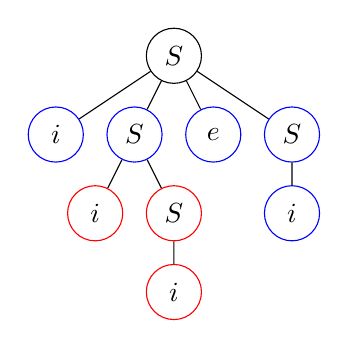
\begin{tikzpicture}[
      level distance=10mm, 
      level 1/.style={sibling distance=10mm},
      level 2/.style={sibling distance=10mm},
      every node/.style={draw, circle, minimum size=7mm, inner sep=2pt},
      color1/.style={draw=red},
      color2/.style={draw=blue}
    ]
    \node {$S$}
        child { node[color2]{$i$} }
        child { node[color2]{$S$}
            child { node[color1]{$i$} }
            child { node[color1]{$S$}
                child { node[color1]{$i$} }
            }
        }
        child { node[color2]{$e$} }
        child { node[color2]{$S$}
            child { node[color2]{$i$} }
        }
    ;
    \end{tikzpicture}
\end{tikzpicture}
\end{center}
\vspace{-40mm}
\subsection{作业2.3}
\subsubsection{题目描述}
类Lisp 程序文法
\begin{align*}
    G[E]:\;\; &E \rightarrow(A, E, E)\;|\;i\\
    &A \rightarrow+\;|\;-\;|\;\times\;|\;{\div}
\end{align*}
\begin{enumerate}
\item 任意变量与  $i$  匹配,  $(\theta, a, b)$  表示  $a \theta b$  的结果,其中  $\theta$  为运算符,试写出  $a \times(b+c)  {\div} d$  的类Lisp 程序形式;
\item 画出上述句子的语法树;
\item 写出上述句子的短语、直接短语和句柄。
\end{enumerate}
\subsubsection{解答}

\paragraph{题目2.3.1} 首先不难画出 $a \times(b+c)  {\div} d$ 的表达式树:


\begin{center} 
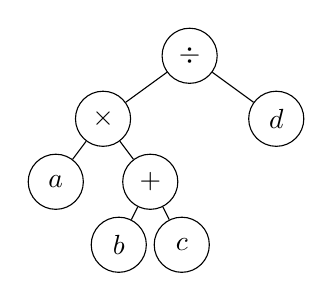
\begin{tikzpicture}[
  level distance=8mm, % 调整上下两行的间隔
  level 1/.style={sibling distance=22mm},
  level 2/.style={sibling distance=12mm},
  level 3/.style={sibling distance=8mm},
  every node/.style={draw, circle, minimum size=7mm, inner sep=2pt},
  ]

% Root node
\node{${\div}$}
    child { node{$\times$}
        child { node{$a$} }
        child { node{$+$}
            child { node{$b$} }
            child { node{$c$} }
        }
    }
    child { node{$d$} };

\end{tikzpicture}
\end{center} 

于是可以写出类Lisp程序形式(实际上是前序遍历的形式?)为:$({\div},(\times,a,(+,b,c)),d)$。

\paragraph{题目2.3.2} 根据上面的程序形式可以写出推导过程:

\begin{align*}
E & \Rightarrow (A,E,E)\\
& \Rightarrow (\div, (A,E,E), d)\\
& \Rightarrow (\div, (\times, a, (A,E,E)), d) \\
& \Rightarrow (\div, (\times, a, (+,b,c)), d)
\end{align*}

不难画出语法树:

\begin{center} 
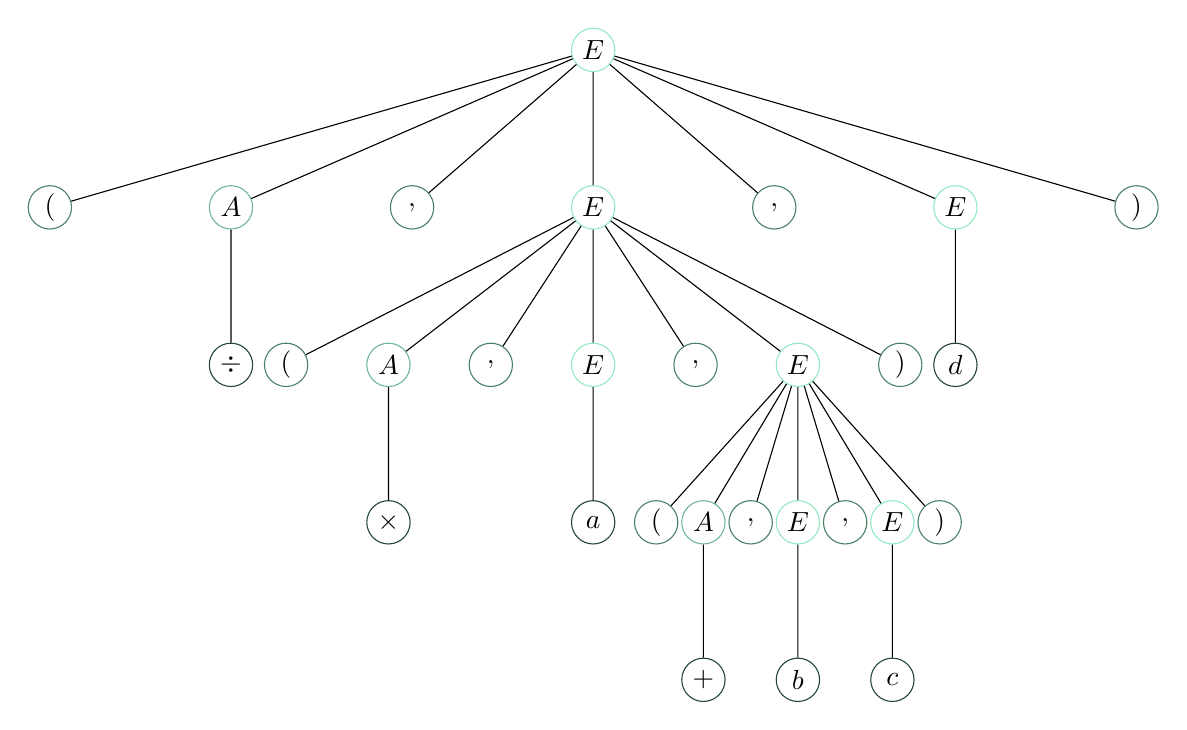
\begin{tikzpicture}[
  level distance=20mm, % 调整上下两行的间隔
  level 1/.style={sibling distance=23mm},
  level 2/.style={sibling distance=13mm},
  level 3/.style={sibling distance=6mm},
  every node/.style={draw, circle, minimum size=5.5mm, inner sep=1pt},
  NodeE/.style={draw=EE},
  NodeA/.style={draw=TT},
  leaf1/.style={draw=FF},
  leaf2/.style={draw=oo},
  ]


\node[NodeE]{$E$}
    child { node[leaf1]{$($} }
    child { node[NodeA]{$A$}
        child { node[leaf2]{$\div$} }
    }
    child { node[leaf1]{$,$} }
    child { node[NodeE]{$E$}
        child { node[leaf1]{$($} }
        child { node[NodeA]{$A$}
            child { node[leaf2]{$\times$} }
        }
        child { node[leaf1]{$,$} }
        child { node[NodeE]{$E$}
            child { node[leaf2]{$a$} }
        }
        child { node[leaf1]{$,$} }
        child { node[NodeE]{$E$}
            child { node[leaf1]{$($} }
            child { node[NodeA]{$A$}
                child { node[leaf2]{$+$} }
            }
            child { node[leaf1]{$,$} }
            child { node[NodeE]{$E$}
                child { node[leaf2]{$b$} }
            }
            child { node[leaf1]{$,$} }
            child { node[NodeE]{$E$}
                child { node[leaf2]{$c$} }
            }
            child { node[leaf1]{$)$} }
        }
        child { node[leaf1]{$)$} }
    }
    child { node[leaf1]{$,$} }
    child { node[NodeE]{$E$}
        child { node[leaf2]{$d$} }
    }
    child { node[leaf1]{$)$} };

\end{tikzpicture}
\end{center} 

\paragraph{题目2.3.3} 根据上图看图写话:

\begin{enumerate}
    \item 短语:$\color{TT}({\div},(\times,a,(+,b,c)),d)$、$\color{FF}($、$\color{oo}{\div}$、$\color{FF},$、$\color{TT}(\times,a,(+,b,c))$、$\color{oo}d$、$\color{FF})$、$\color{oo}\times$、$\color{oo}a$、$\color{TT}(+,b,c)$、$\color{oo}+$、$\color{oo}b$、$\color{oo}c$;
    \item 直接短语:$\color{oo}\div$、$\color{oo}\times$、$\color{oo}a$、$\color{oo}+$、$\color{oo}b$、$\color{oo}c$、$\color{oo}d$;
    \item 句柄:$\color{oo}\div$。
\end{enumerate}

\newpage
	% 代码分析:模块功能、涉及到的类、类关系、数据结构及关键代码等;
	% 任务要求,设计任务要求;
	% 设计:详细的设计方案,相关的数据结构、算法描述,可采用伪代码等形式化描述
	% 实现:修改哪些类、如何修改、为什么修改等;
	% 测试:测试用例,测试结果及结果分析,测试运行界面等;
	% 调试:调试方法,遇到的问题及解决方案等;
	% 结论与展望:完成的主要工作、收获、进一步的工作,建议、体会、心得等;

\section{作业3}
\subsection{作业3.1}
\subsubsection{题目描述}

C 风格变量声明的正规式:

\[(i|r)v(,v)^*;\]

其中 $i$ 和 $r$ 分别表示整型和实型数据类型,$v$ 表示变量名。

\begin{enumerate}
    \item 构造NFA,并单符化。
    \item 确定化。
    \item 最小化。
\end{enumerate}

\subsubsection{解答}

\paragraph{构造NFA,并单符化。} 按照给出的步骤,不难画出:

\begin{figure}[H]
    \centering
    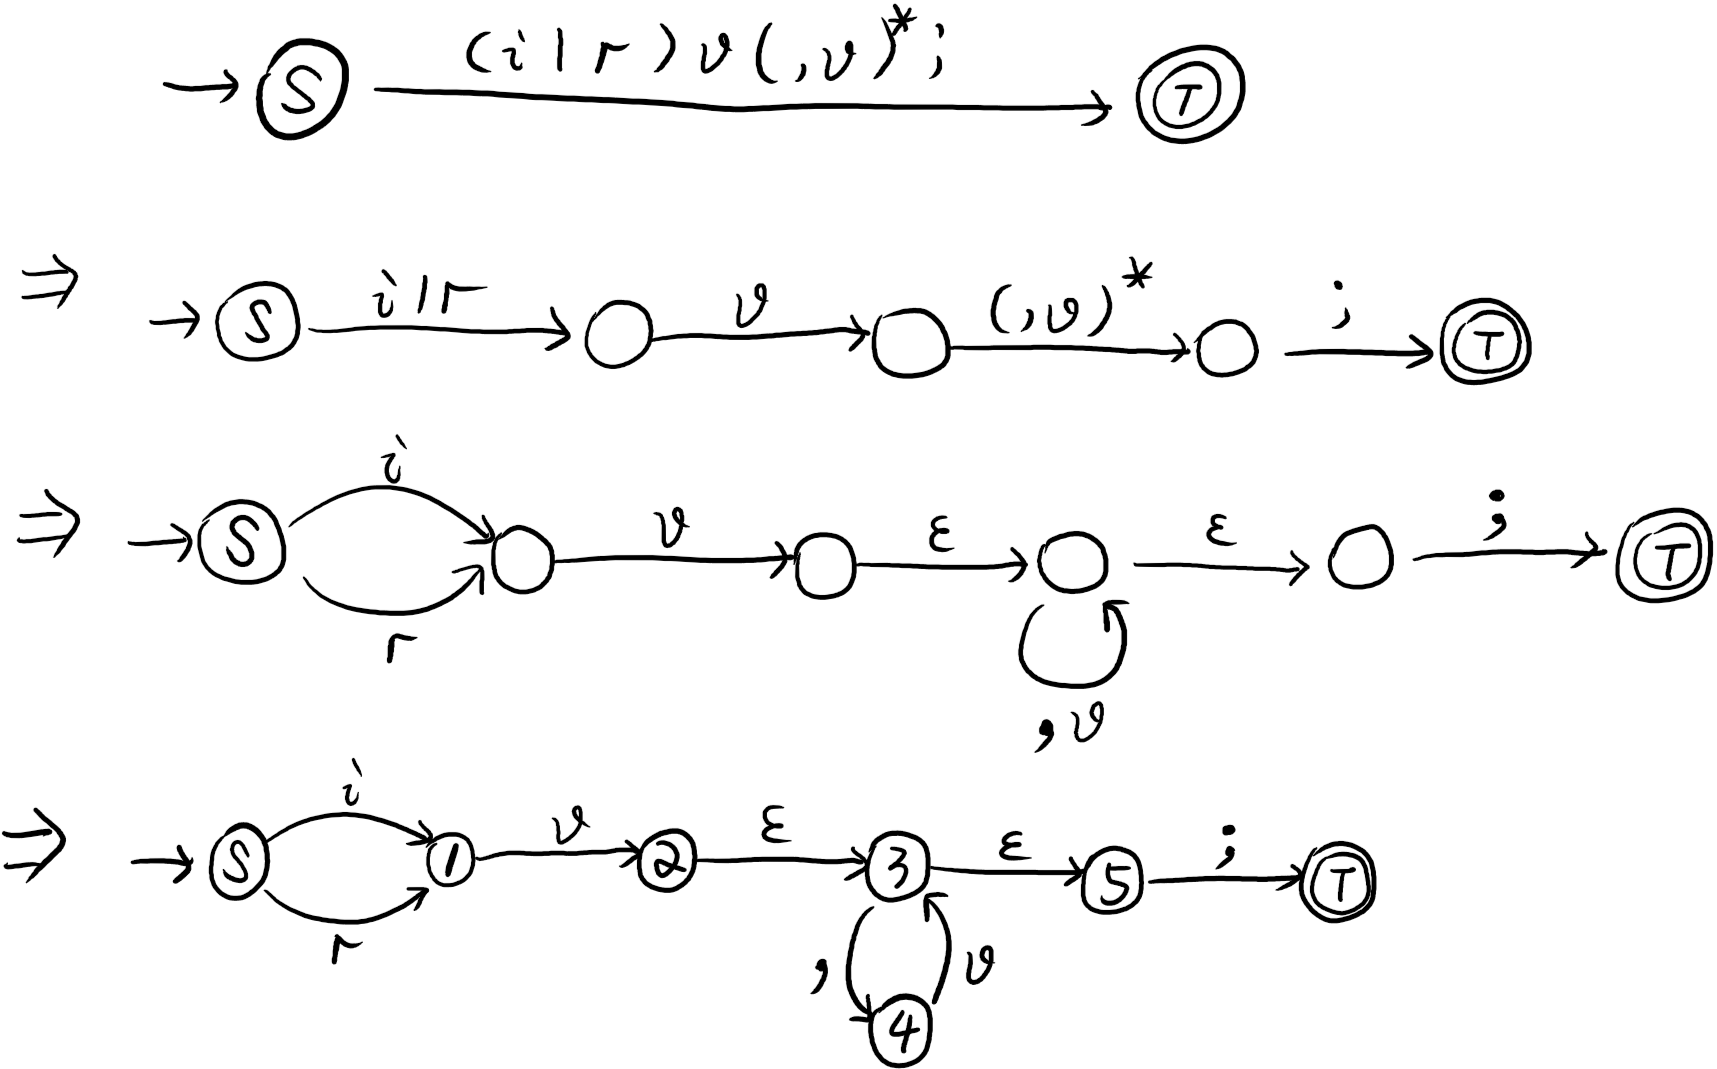
\includegraphics[width=0.8\linewidth]{imgs/3.png}
    \caption{正则 $r$ $\Rightarrow\;$NFA $M$}
    \label{fig:NFA}
\end{figure}

\paragraph{确定化。} 对于上面画出的NFA,首先设字母表为 $\Sigma=\left\{i,r,',',v,';'\right\}$,初态为 $X$,可以写出闭包:

\begin{center}
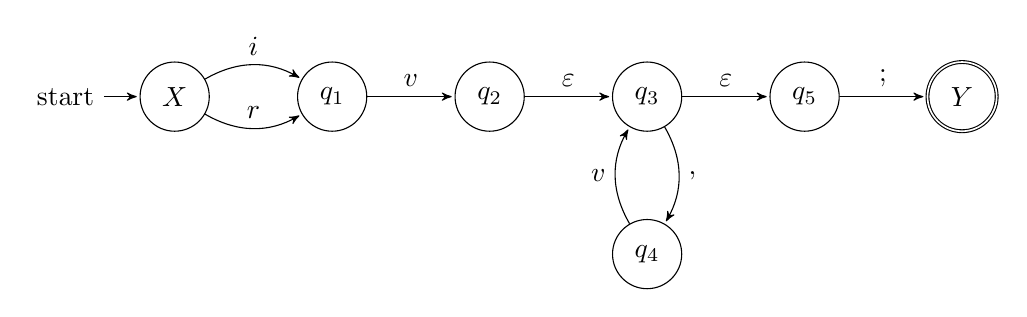
\begin{tikzpicture}[>=stealth',shorten >=1pt,auto,node distance=2cm]
  \node[initial,state] (X)      {$X$};
  \node[state]         (q1) [right of=X]  {$q_1$};
  \node[state]         (q2) [right of=q1] {$q_2$};
  \node[state]         (q3) [right of=q2] {$q_3$};
  \node[state]         (q4) [below of=q3] {$q_4$};
  \node[state]         (q5) [right of=q3] {$q_5$};
  \node[state,accepting](Y) [right of=q5] {$Y$};

  \path[->]  (X)  edge[bend right] node {$r$} (q1);
  \path[->]  (X)  edge[bend left] node {$i$} (q1);
  \path[->]  (q1)  edge node {$v$} (q2);
  \path[->]  (q2)  edge node {$\varepsilon$} (q3);
  \path[->]  (q3)  edge node {$\varepsilon$} (q5);
  \path[->]  (q5)  edge node {$;$} (Y);
  \path[->]  (q3)  edge[bend left] node {$,$} (q4);
  \path[->]  (q4)  edge[bend left] node {$v$} (q3);
\end{tikzpicture}
\end{center}


\begin{table}[H]
    \centering
    \begin{tabular}{>{\bfseries}c *5{c}}
        \toprule
        $I$ & $I_r$ & $I_i$ & $I_v$ & $I_,$ & $I_;$\\
        \midrule
        $\{X\}$ & $\{q_1\}$ & $\{q_1\}$ & $\Phi$ & $\Phi$ & $\Phi$\\
        $\{q_1\}$ & $\Phi$ & $\Phi$ & $\{q_2, q_3, q_5\}$ & $\Phi$ & $\Phi$\\
        $\{q_2, q_3, q_5\}$ & $\Phi$ & $\Phi$ & $\Phi$ & $\{q_4\}$ & $\{Y\}$\\
        $\{q_4\}$ & $\Phi$ & $\Phi$ & $\{q_3, q_5\}$ & $\Phi$ & $\Phi$\\
        $\{q_3, q_5\}$ & $\Phi$ & $\Phi$ & $\Phi$ & $\{q_4\}$ & $\{Y\}$\\
        $\{Y\}$ & $\Phi$ & $\Phi$ & $\Phi$ & $\Phi$ & $\Phi$\\
        \bottomrule
    \end{tabular}
    \caption{$\delta^\prime:\; S\times\Sigma\to S$}
    \label{tab:my_label}
\end{table}

可以按次序编号为:

\begin{table}[H]
    \centering
    \begin{tabular}{>{\bfseries}c *5{c}}
        \toprule
        $I$ & $I_r$ & $I_i$ & $I_v$ & $I_,$ & $I_;$\\
        \midrule
        $S$ & $1$ & $1$ &  &  & \\
        $1$ &  &  & $2$ &  & \\
        $2$ &  &  &  & $3$ & $T$\\
        $3$ &  &  & $4$ &  & \\
        $4$ &  &  &  & $3$ & $T$\\
        $T$ &  &  &  &  & \\
        \bottomrule
    \end{tabular}
    \caption{$\delta^\prime:\; S\times\Sigma\to S$}
    \label{tab:my_label}
\end{table}

根据 $\delta^\prime$ 可以画出:

\begin{center}
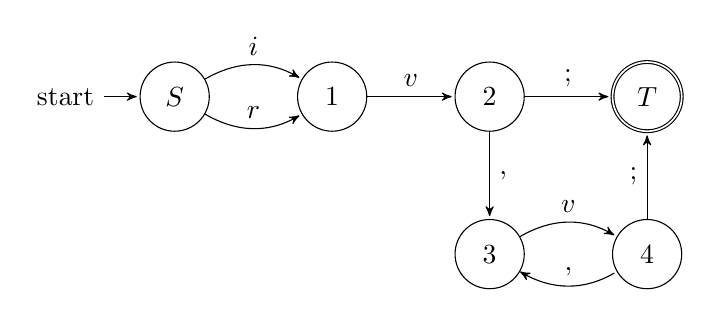
\begin{tikzpicture}[>=stealth',shorten >=1pt,auto,node distance=2cm]
  \node[initial,state] (X)      {$S$};
  \node[state]         (q1) [right of=X]  {$1$};
  \node[state]         (q235) [right of=q1] {$2$};
  \node[state]         (q4) [below of=q235] {$3$};
  \node[state]         (q35) [right of=q4] {$4$};
  \node[state,accepting](Y) [right of=q235] {$T$};

  \path[->]  (X)  edge[bend right] node {$r$} (q1);
  \path[->]  (X)  edge[bend left] node {$i$} (q1);
  \path[->]  (q1)  edge node {$v$} (q235);
  \path[->]  (q235)  edge node {$;$} (Y);
  \path[->]  (q235)  edge node {$,$} (q4);
  \path[<-]  (q4)  edge[bend right] node {$,$} (q35);
  \path[->]  (q4)  edge[bend left] node {$v$} (q35);
  \path[->]  (q35)  edge node {$;$} (Y);
\end{tikzpicture}
\end{center}

\paragraph{最小化。} 在上表中可以看出 2 与 4 对应的列完全相同,故其为等价状态,可以合并为:

\begin{center}
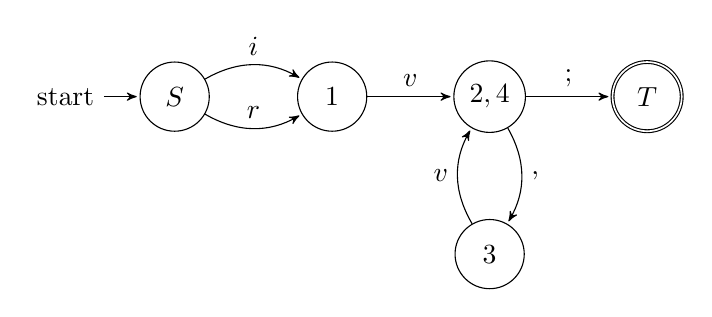
\begin{tikzpicture}[>=stealth',shorten >=1pt,auto,node distance=2cm]
  \node[initial,state] (X)      {$S$};
  \node[state]         (q1) [right of=X]  {$1$};
  \node[state]         (q235) [right of=q1] {$2,4$};
  \node[state]         (q4) [below of=q235] {$3$};
  \node[state,accepting](Y) [right of=q235] {$T$};

  \path[->]  (X)  edge[bend right] node {$r$} (q1);
  \path[->]  (X)  edge[bend left] node {$i$} (q1);
  \path[->]  (q1)  edge node {$v$} (q235);
  \path[->]  (q235)  edge node {$;$} (Y);
  \path[->]  (q235)  edge[bend left] node {$,$} (q4);
  \path[->]  (q4)  edge[bend left] node {$v$} (q235);
\end{tikzpicture}
\end{center}

此时将 $2,4$ 编号为 $2^\prime$,编号表格为:

\begin{table}[H]
    \centering
    \begin{tabular}{>{\bfseries}c *5{c}}
        \toprule
        $I$ & $I_r$ & $I_i$ & $I_v$ & $I_,$ & $I_;$\\
        \midrule
        $S$ & $1$ & $1$ &  &  & \\
        $1$ &  &  & $2^\prime$ &  & \\
        $2^\prime$ &  &  &  & $3$ & $T$\\
        $3$ &  &  & $2^\prime$ &  & \\
        $T$ &  &  &  &  & \\
        \bottomrule
    \end{tabular}
    \caption{$\delta^\prime:\; S\times\Sigma\to S$}
    \label{tab:my_label}
\end{table}

可以看到 $1$ 与 $3$ 完全相同,记为 $1^\prime$,可以化简为:

\begin{center}
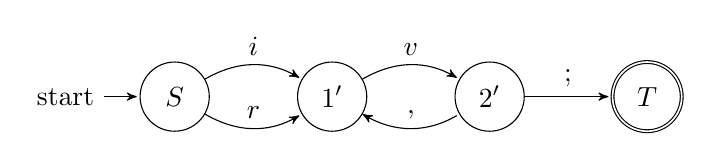
\begin{tikzpicture}[>=stealth',shorten >=1pt,auto,node distance=2cm]
  \node[initial,state] (X)      {$S$};
  \node[state]         (q1) [right of=X]  {$1^\prime$};
  \node[state]         (q235) [right of=q1] {$2^\prime$};
  \node[state,accepting](Y) [right of=q235] {$T$};

  \path[->]  (X)  edge[bend right] node {$r$} (q1);
  \path[->]  (X)  edge[bend left] node {$i$} (q1);
  \path[->]  (q1)  edge[bend left] node {$v$} (q235);
  \path[<-]  (q1)  edge[bend right] node {$,$} (q235);
  \path[->]  (q235)  edge node {$;$} (Y);
\end{tikzpicture}
\end{center}

此时编号表格为:

\begin{table}[H]
    \centering
    \begin{tabular}{>{\bfseries}c *5{c}}
        \toprule
        $I$ & $I_r$ & $I_i$ & $I_v$ & $I_,$ & $I_;$\\
        \midrule
        $S$ & $1$ & $1$ &  &  & \\
        $1^\prime$ &  &  & $2^\prime$ &  & \\
        $2^\prime$ &  &  &  & $3$ & $T$\\
        $T$ &  &  &  &  & \\
        \bottomrule
    \end{tabular}
    \caption{$\delta^\prime:\; S\times\Sigma\to S$}
    \label{tab:my_label}
\end{table}


每列有且仅有一种转移,是最小化的充分条件,故此时为最小化 DFA。

% \subsection{作业1.2}
% \subsubsection{题目描述}
% \subsubsection{解答}

% \subsection{作业1.3}
% \subsubsection{题目描述}
% \subsubsection{解答}

\newpage
	% 代码分析:模块功能、涉及到的类、类关系、数据结构及关键代码等;
	% 任务要求,设计任务要求;
	% 设计:详细的设计方案,相关的数据结构、算法描述,可采用伪代码等形式化描述
	% 实现:修改哪些类、如何修改、为什么修改等;
	% 测试:测试用例,测试结果及结果分析,测试运行界面等;
	% 调试:调试方法,遇到的问题及解决方案等;
	% 结论与展望:完成的主要工作、收获、进一步的工作,建议、体会、心得等;

\section{作业4}
\subsection{作业4.1}
\subsubsection{题目描述}

将右线性文法$G[S]: S \rightarrow xA\;|\;yB\;|\;\varepsilon\;,\;A \rightarrow yA\;|\;y\;,\;B \rightarrow xB\;|\;x$, 转换为:
\begin{enumerate}
    \item 有限自动机。
    \item 正则式。
\end{enumerate}

\subsubsection{解答}

\paragraph{有限自动机。} 令有限自动机 $M=\left(\{S,A,B,f\},\{x,y\},\delta,\{S\},\{f\}\right)$,其中 $f$ 为添加的终态符号。

类似例题 3.15 的步骤,构造 $\delta$:

\begin{enumerate}
    \item 对于产生式 $S \rightarrow xA$,由 $S$ 向 $A$ 引 $x$ 弧。
    \item 对于产生式 $S \rightarrow yB$,由 $S$ 向 $B$ 引 $y$ 弧。
    \item 对于产生式 $S \rightarrow \varepsilon$,由 $S$ 向 $f$ 引 $\varepsilon$ 弧。
    \item ...
\end{enumerate}

不难画出:

\begin{center}
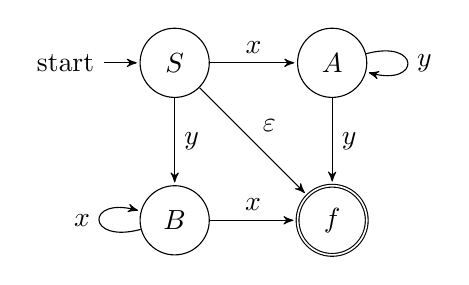
\begin{tikzpicture}[>=stealth',shorten >=1pt,auto,node distance=2cm]
  \node[initial,state] (S)      {$S$};
  \node[state]         (A) [right of=S]  {$A$};
  \node[state]         (B) [below of=S] {$B$};
  \node[state,accepting](f) [below of=A] {$f$};

  \path[->]  (S)  edge node {$x$} (A);
  \path[->]  (S)  edge node {$y$} (B);
  \path[->]  (S)  edge node {$\varepsilon$} (f);
  \path[->]  (A)  edge[loop right] node {$y$} (A);
  \path[->]  (B)  edge[loop left] node {$x$} (B);
  \path[->]  (A)  edge node {$y$} (f);
  \path[->]  (B)  edge node {$x$} (f);
\end{tikzpicture}
\end{center}

\paragraph{正规式} 正规式可以直接与线性文法转换,于是就不借助有限自动机了(虽然这个题使用自动机转换也很简单)。

首先改写:

\begin{enumerate}
    \item $S \rightarrow xA\;|\;yB\;|\;\varepsilon\;$ 不包含本身,直接写为:$S \rightarrow (xA|yB|\varepsilon)$;
    \item $A \rightarrow yA\;|\;y\;$ 改写为 $A \rightarrow (yA|y)$,也就是 $A\rightarrow y^*y$,$B$ 完全同理,改写为 $B\rightarrow x^*x$;
    \item 将第二步的结果代入第一步,得到 $S \rightarrow (xy^*y|yx^*x|\varepsilon)$。
\end{enumerate}

最终得到正规式为 $(xy^*y|yx^*x|\varepsilon)$,如果允许使用 $+$ 与 $?$,可以简写为 $(xy^+|yx^+)?$。

\subsection{作业4.2}
\subsubsection{题目描述}
给定右线性文法$G[S]$, 求其等价的左线性文法:
\begin{align*}
    S&\rightarrow 0S\;|\;1S\;|\;1A\;|\;0B\\
    A&\rightarrow 1C\;|\;1\\
    B&\rightarrow 0C\;|\;0\\
    C&\rightarrow 0C\;|\;1C\;|\;0\;|\;1
\end{align*}
\subsubsection{解答}

字符数较少,似乎用正则比较方便?,下面通过右线性文法转正规式,再将正规式转左线性文法来实现转换:

\paragraph{转正规式} 与上题类似,首先改写:(下方便起见,记$\Sigma=\{0,1\}$)

\begin{itemize}
    \item $S\rightarrow 0S\;|\;1S\;|\;1A\;|\;0B$ 首先写为 $S\rightarrow (\Sigma S|1A|0B)$,也就是 $S\rightarrow \Sigma^*(1A|0B)$;
    \item $A\rightarrow 1C\;|\;1$ 简写为 $A\rightarrow 1C?$,$B$ 同理简写为 $0C?$;
    \item $C\rightarrow 0C\;|\;1C\;|\;0\;|\;1$ 首先写为 $C\rightarrow (\Sigma C|\Sigma)$,也就是 $\Sigma^+$;
    \item 依次代入上面式子,得到 $S\rightarrow \Sigma^*(11|00)\Sigma^+?$
\end{itemize}

得到正规式为 $(0|1)^*(11|00)(((1|0)(1|0)^*)|\varepsilon)$。

\paragraph{左线性文法} 类似上文,进行逐步拆解:

\begin{enumerate}
    \item ${\color{Red} \Sigma^*} ({\color{Purple} 11} |{\color{Orange} 00} ){\color{Green} \Sigma^+ ?} $ 替换为 $S\rightarrow S_1 {\color{Green} \Sigma^+ ?}$、$S_1\rightarrow S_2{\color{Purple} 1}|S_3{\color{Orange} 0}$、$S_2\rightarrow S_4{\color{Purple} 1}$、$S_3\rightarrow S_4{\color{Orange} 0}$、$S_4\rightarrow {\color{Red} \Sigma^*}$;
    \item $S\rightarrow S_1 \Sigma^+?$ 可写为 $S\rightarrow S_1 0\;|\;S_11\;|\;S0\;|\;S1$;
    \item $S_4\rightarrow \Sigma^*$ 可写为 $S_4\rightarrow S_40\;|\;S_41\;|\;0\;|\;1\;|\;\varepsilon$;
\end{enumerate}

总伤,该正规式 ${\color{Red} \Sigma^*} ({\color{Purple} 11} |{\color{Orange} 00} ){\color{Green} \Sigma^+ ?} $,也就是给出的右线性文法对应的左线性文法为:

\begin{align*}
    S&\rightarrow {\color{Purple} S_21} \;|\;{\color{Orange} S_30} \;|\;{\color{Green} S_1 0\;|\;S_11\;|\;S0\;|\;S1} \\
    S_1&\rightarrow {\color{Purple} S_21} \;|\;{\color{Orange} S_30} \\
    S_2&\rightarrow {\color{Purple} S_41} \\
    S_3&\rightarrow {\color{Orange} S_40} \\
    S_4&\rightarrow {\color{Red} S_40\;|\;S_41\;|\;0\;|\;1\;|\;\varepsilon} 
\end{align*}

\newpage
	% 代码分析:模块功能、涉及到的类、类关系、数据结构及关键代码等;
	% 任务要求,设计任务要求;
	% 设计:详细的设计方案,相关的数据结构、算法描述,可采用伪代码等形式化描述
	% 实现:修改哪些类、如何修改、为什么修改等;
	% 测试:测试用例,测试结果及结果分析,测试运行界面等;
	% 调试:调试方法,遇到的问题及解决方案等;
	% 结论与展望:完成的主要工作、收获、进一步的工作,建议、体会、心得等;

\section{作业5}
\subsection{作业5.1}
\subsubsection{题目描述}
C风格声明语句文法为 \(G\left\lbrack L\right\rbrack = \left( {\{ L,D,T\} ,\{ ;,,,\text{id,int,double}\} ,P,L}\right)\) ,产生式如下:

\(L \rightarrow L;D\) $\quad$ \(L \rightarrow D\) $\quad$ \(D \rightarrow T \;id\) $\quad$ \(D \rightarrow D,{id}\quad T \rightarrow\) int $\quad$ \(T \rightarrow\) double

\begin{enumerate}
    \item 消除文法产生式的左递归;
    \item 构造所有非终结符号的首符集 First;
    \item 构造所有非终结符号的后继符集 Follow;
    \item 构造 $LL(1)$ 分析表;
    \item 给出句子int \(i\) ; double \(x,y\) 的分析过程。
\end{enumerate}

\subsubsection{解答}

\paragraph{消除文法产生式的左递归} 转为右递归文法:

\(L \rightarrow L;D\) $\quad$ \(L \rightarrow D\) 替换为:

\begin{itemize}
    \item $L \rightarrow  D{L}^{\prime }$
    \item ${L}^{\prime } \rightarrow  ;D{L}^{\prime } \mid  \varepsilon$
\end{itemize}

\(D \rightarrow T \;id\) $\quad$ \(D \rightarrow D,{id}\) 替换为:

\begin{itemize}
    \item $D \rightarrow T\;id\;{D}^{\prime }$
    \item ${D}^{\prime } \rightarrow ,id$ ${D}^{\prime } \mid  \varepsilon$
\end{itemize}

\paragraph{First} 可以直接写出:

\begin{lstlisting}[language=c++,title={First},mathescape]
First($T$)={int, double}
First(${D}$)={, , $\varepsilon$}
First(${D}^{\prime }$)={int, double}
First(${L}^{\prime }$)={; , $\varepsilon$}
First($L$)={int, double}
\end{lstlisting}

\paragraph{Follow} 由于不存在隐式左递归,可以整理为:

\begin{itemize}
    \item $L \rightarrow  D{L}^{\prime }$
    \item ${L}^{\prime } \rightarrow  ;D{L}^{\prime } \mid  \varepsilon$
    \item $D \rightarrow  T\;{id\; D}^{\prime }$
    \item ${D}^{\prime } \rightarrow,id\;{D}^{\prime }$ | ${\varepsilon }$
    \item $T \rightarrow$ int | double
\end{itemize}

\begin{lstlisting}[language=c++,title={Follow},mathescape]
First($T$)={id, #}
First(${D}$)={; , #}
First(${D}^{\prime }$)={; , #}
First(${L}^{\prime }$)={#}
First($L$)={#}
\end{lstlisting}

\paragraph{LL(1) 分析表} 不难画出:



\begin{table}[htbp]
\centering
\renewcommand{\arraystretch}{1.2} % 增加行间距
\setlength{\tabcolsep}{10pt}      % 设置列间距
\caption{LL(1) 分析表}
\label{tab:LL1}
\begin{tabularx}{\textwidth}{>{\centering\arraybackslash}Xcccccc}
\toprule
 & , & ; & $id$ & int & double & $\#$ \\
\midrule
$L$ &  &  &  & $\#L \rightarrow DL^{\prime}$ & $\#L \rightarrow DL^{\prime}$ & \\
\rowcolor[gray]{.9} % 使用灰色背景以区分不同行
$L^{\prime}$ &  & $\#L^{\prime} \rightarrow ;DL^{\prime}$ &  &  &  & $\#L^{\prime} \rightarrow \varepsilon$\\
$D$ &  &  &  & $D \rightarrow T\;id\;D^\prime$ & $D \rightarrow T\;id\;D^\prime$ & \\
\rowcolor[gray]{.9}
$D^{\prime}$ & $D^{\prime} \rightarrow,id\;D^{\prime}$ & $D^{\prime} \rightarrow \varepsilon$ &  &  &  & $D^{\prime} \rightarrow \varepsilon$\\
$T$ &  &  &  & $T \rightarrow$ int & $T \rightarrow$ double & \\
\bottomrule
\end{tabularx}
\end{table}

\paragraph{int i; double x,y 分析过程:} 可以写出:


\begin{center}
\begin{tabular}{rl@{\hspace{10em}}r}
1 & $\#E$ & int $i$; double $x,y\#$ \\
\hline
2 & $\#L^\prime D^\prime$ & int $i$; double $x,y\#$ \\
\hline
3 & $\#L^\prime D^\prime\;id\;T$ & int $i$; double $x,y\#$ \\
\hline
4 & $\#L^\prime D^\prime\;id\;$ int & int $i$; double $x,y\#$ \\
\hline
5 & $\#L^\prime D^\prime\;id\;$ & $i$; double $x,y\#$ \\
\hline
6 & $\#L^\prime D^\prime$ & ; double $x,y\#$ \\
\hline
7 & $\#L^\prime$ & ; double $x,y\#$ \\
\hline
8 & $\#L^\prime D;$ & ; double $x,y\#$ \\
\hline
9 & $\#L^\prime D$ & double $x,y\#$ \\
\hline
10 & $\#L^\prime D^\prime\;id\;T$ & double $x,y\#$ \\
\hline
11 & $\#L^\prime D^\prime\;id$ double & double $x,y\#$ \\
\hline
12 & $\#L^\prime D^\prime\;id$ & $x,y\#$ \\
\hline
13 & $\#L^\prime D^\prime$ & $,y\#$ \\
\hline
14 & $\#L^\prime D^\prime\;id,$ & $,y\#$ \\
\hline
15 & $\#L^\prime D^\prime\;id$ & $y\#$ \\
\hline
16 & $\#L^\prime D^\prime$ & $\#$\\
\hline
17 & $\#L^\prime$ & $\#$\\
\hline
18 & $\#$ & $\#$\\
\end{tabular}
\end{center}

\newpage
	% 代码分析:模块功能、涉及到的类、类关系、数据结构及关键代码等;
	% 任务要求,设计任务要求;
	% 设计:详细的设计方案,相关的数据结构、算法描述,可采用伪代码等形式化描述
	% 实现:修改哪些类、如何修改、为什么修改等;
	% 测试:测试用例,测试结果及结果分析,测试运行界面等;
	% 调试:调试方法,遇到的问题及解决方案等;
	% 结论与展望:完成的主要工作、收获、进一步的工作,建议、体会、心得等;

\section{作业6}

文法 $G[E]:\;E \rightarrow E \operatorname{o} E \;|\; E E \;|\; E * \;|\; (E) \;|\; i$ 是生成正规式的二义文法,为了避免与文法元语言符号 “|” 冲突,或运算用符号 $\operatorname{o}$ 表示;连接运算则省略; $∗$ 为闭包运算;$i$ 表示单词,既任何表示单词的终结符号均可与之匹配:
\begin{enumerate}
    \item 构造 LR(1) 项目集规范族;
    \item 构造 LR(1) 分析表,如有冲突,请根据正规式的运算规则消除之;
    \item 用 LR(1) 分析表分析有两个连续 $a$ 或两个连续 $b$ 的句子:$(a\operatorname{o}b)*(aa\operatorname{o}bb)(a\operatorname{o}b)*$。
\end{enumerate}

\subsection{作业6.1}

首先拓广文法,加入 $S\rightarrow E$,不难写出 First 与 Follow:

\begin{itemize}
    \item E:First=\{(, $i$\}、Follow=\{ \#, o, (, $i$, * \}
    \item S:First=\{(, $i$\}、Follow=\{ \# \}
\end{itemize}

首先尝试直接转换:

\begin{center}
    \centering
    \begin{longtable}{r|ccc}

\toprule
State &       Items        &         Lookaheads          &  Transitions  \\
\hline
0     &  S $\rightarrow$ . E          & \{ \# \}                       &   E   $\rightarrow$  1   \\
      &  E $\rightarrow$ . E o E    & \{ \#, o, (, $i$, * \}   &  (  $\rightarrow$  2   \\
      &  E $\rightarrow$ . E E        & \{ \#, o, (, $$i$$, * \}   &  $i$  $\rightarrow$  3   \\
      &  E $\rightarrow$ . E *      & \{ \#, o, (, $i$, * \}   &               \\
      &  E $\rightarrow$ . ( E )  & \{ \#, o, (, $i$, * \}   &               \\
      &  E $\rightarrow$ . $i$        & \{ \#, o, (, $i$, * \}   &               \\
\hline
1     &  S $\rightarrow$ E .          & \{ \# \}                       &  (  $\rightarrow$  2   \\
      &  E $\rightarrow$ E . o E    & \{ \#, o, (, $i$, * \}   &  $i$  $\rightarrow$  3   \\
      &  E $\rightarrow$ E . E        & \{ \#, o, (, $i$, * \}   &   E   $\rightarrow$  14  \\
      &  E $\rightarrow$ E . *      & \{ \#, o, (, $i$, * \}   &  *  $\rightarrow$  15  \\
      &  E $\rightarrow$ . E o E    & \{ \#, o, (, $i$, * \}   &  o  $\rightarrow$  16  \\
      &  E $\rightarrow$ . E E        & \{ \#, o, (, $i$, * \}   &               \\
      &  E $\rightarrow$ . E *      & \{ \#, o, (, $i$, * \}   &               \\
      &  E $\rightarrow$ . ( E )  & \{ \#, o, (, $i$, * \}   &               \\
      &  E $\rightarrow$ . $i$        & \{ \#, o, (, $i$, * \}   &               \\
\hline
2     &  E $\rightarrow$ ( . E )  & \{ \#, o, (, $i$, * \}   &   E   $\rightarrow$  4   \\
      &  E $\rightarrow$ . E o E    & \{ ), o, (, $i$, * \} &  (  $\rightarrow$  5   \\
      &  E $\rightarrow$ . E E        & \{ ), o, (, $i$, * \} &  $i$  $\rightarrow$  6   \\
      &  E $\rightarrow$ . E *      & \{ ), o, (, $i$, * \} &               \\
      &  E $\rightarrow$ . ( E )  & \{ ), o, (, $i$, * \} &               \\
      &  E $\rightarrow$ . $i$        & \{ ), o, (, $i$, * \} &               \\
\hline
3     &  E $\rightarrow$ $i$ .        & \{ \#, o, (, $i$, * \}   &               \\
\hline
4     &  E $\rightarrow$ ( E . )  & \{ \#, o, (, $i$, * \}   &  (  $\rightarrow$  5   \\
      &  E $\rightarrow$ E . o E    & \{ ), o, (, $i$, * \} &  $i$  $\rightarrow$  6   \\
      &  E $\rightarrow$ E . E        & \{ ), o, (, $i$, * \} &   E   $\rightarrow$  9   \\
      &  E $\rightarrow$ E . *      & \{ ), o, (, $i$, * \} &  *  $\rightarrow$  10  \\
      &  E $\rightarrow$ . E o E    & \{ ), o, (, $i$, * \} &  o  $\rightarrow$  11  \\
      &  E $\rightarrow$ . E E        & \{ ), o, (, $i$, * \} &  )  $\rightarrow$  13  \\
      &  E $\rightarrow$ . E *      & \{ ), o, (, $i$, * \} &               \\
      &  E $\rightarrow$ . ( E )  & \{ ), o, (, $i$, * \} &               \\
      &  E $\rightarrow$ . $i$        & \{ ), o, (, $i$, * \} &               \\
\hline
5     &  E $\rightarrow$ ( . E )  & \{ ), o, (, $i$, * \} &  (  $\rightarrow$  5   \\
      &  E $\rightarrow$ . E o E    & \{ ), o, (, $i$, * \} &  $i$  $\rightarrow$  6   \\
      &  E $\rightarrow$ . E E        & \{ ), o, (, $i$, * \} &   E   $\rightarrow$  7   \\
      &  E $\rightarrow$ . E *      & \{ ), o, (, $i$, * \} &               \\
      &  E $\rightarrow$ . ( E )  & \{ ), o, (, $i$, * \} &               \\
      &  E $\rightarrow$ . $i$        & \{ ), o, (, $i$, * \} &               \\
\hline
6     &  E $\rightarrow$ $i$ .        & \{ ), o, (, $i$, * \} &               \\
\hline
7     &  E $\rightarrow$ ( E . )  & \{ ), o, (, $i$, * \} &  (  $\rightarrow$  5   \\
      &  E $\rightarrow$ E . o E    & \{ ), o, (, $i$, * \} &  $i$  $\rightarrow$  6   \\
      &  E $\rightarrow$ E . E        & \{ ), o, (, $i$, * \} &  )  $\rightarrow$  8   \\
      &  E $\rightarrow$ E . *      & \{ ), o, (, $i$, * \} &   E   $\rightarrow$  9   \\
      &  E $\rightarrow$ . E o E    & \{ ), o, (, $i$, * \} &  *  $\rightarrow$  10  \\
      &  E $\rightarrow$ . E E        & \{ ), o, (, $i$, * \} &  o  $\rightarrow$  11  \\
      &  E $\rightarrow$ . E *      & \{ ), o, (, $i$, * \} &               \\
      &  E $\rightarrow$ . ( E )  & \{ ), o, (, $i$, * \} &               \\
      &  E $\rightarrow$ . $i$        & \{ ), o, (, $i$, * \} &               \\
\hline
8     &  E $\rightarrow$ ( E ) .  & \{ ), o, (, $i$, * \} &               \\
\hline
9     &  E $\rightarrow$ E E .        & \{ ), o, (, $i$, * \} &  (  $\rightarrow$  5   \\
      &  E $\rightarrow$ E . o E    & \{ ), o, (, $i$, * \} &  $i$  $\rightarrow$  6   \\
      &  E $\rightarrow$ E . E        & \{ ), o, (, $i$, * \} &   E   $\rightarrow$  9   \\
      &  E $\rightarrow$ E . *      & \{ ), o, (, $i$, * \} &  *  $\rightarrow$  10  \\
      &  E $\rightarrow$ . E o E    & \{ ), o, (, $i$, * \} &  o  $\rightarrow$  11  \\
      &  E $\rightarrow$ . E E        & \{ ), o, (, $i$, * \} &               \\
      &  E $\rightarrow$ . E *      & \{ ), o, (, $i$, * \} &               \\
      &  E $\rightarrow$ . ( E )  & \{ ), o, (, $i$, * \} &               \\
      &  E $\rightarrow$ . $i$        & \{ ), o, (, $i$, * \} &               \\
\hline
10    &  E $\rightarrow$ E * .      & \{ ), o, (, $i$, * \} &               \\
\hline
11    &  E $\rightarrow$ E o . E    & \{ ), o, (, $i$, * \} &  (  $\rightarrow$  5   \\
      &  E $\rightarrow$ . E o E    & \{ ), o, (, $i$, * \} &  $i$  $\rightarrow$  6   \\
      &  E $\rightarrow$ . E E        & \{ ), o, (, $i$, * \} &   E   $\rightarrow$  12  \\
      &  E $\rightarrow$ . E *      & \{ ), o, (, $i$, * \} &               \\
      &  E $\rightarrow$ . ( E )  & \{ ), o, (, $i$, * \} &               \\
      &  E $\rightarrow$ . $i$        & \{ ), o, (, $i$, * \} &               \\
\hline
12    &  E $\rightarrow$ E o E .    & \{ ), o, (, $i$, * \} &  (  $\rightarrow$  5   \\
      &  E $\rightarrow$ E . o E    & \{ ), o, (, $i$, * \} &  $i$  $\rightarrow$  6   \\
      &  E $\rightarrow$ E . E        & \{ ), o, (, $i$, * \} &   E   $\rightarrow$  9   \\
      &  E $\rightarrow$ E . *      & \{ ), o, (, $i$, * \} &  *  $\rightarrow$  10  \\
      &  E $\rightarrow$ . E o E    & \{ ), o, (, $i$, * \} &  o  $\rightarrow$  11  \\
      &  E $\rightarrow$ . E E        & \{ ), o, (, $i$, * \} &               \\
      &  E $\rightarrow$ . E *      & \{ ), o, (, $i$, * \} &               \\
      &  E $\rightarrow$ . ( E )  & \{ ), o, (, $i$, * \} &               \\
      &  E $\rightarrow$ . $i$        & \{ ), o, (, $i$, * \} &               \\
\hline
13    &  E $\rightarrow$ ( E ) .  & \{ \#, o, (, $i$, * \}   &               \\
\hline
14    &  E $\rightarrow$ E E .        & \{ \#, o, (, $i$, * \}   &  (  $\rightarrow$  2   \\
      &  E $\rightarrow$ E . o E    & \{ \#, o, (, $i$, * \}   &  $i$  $\rightarrow$  3   \\
      &  E $\rightarrow$ E . E        & \{ \#, o, (, $i$, * \}   &   E   $\rightarrow$  14  \\
      &  E $\rightarrow$ E . *      & \{ \#, o, (, $i$, * \}   &  *  $\rightarrow$  15  \\
      &  E $\rightarrow$ . E o E    & \{ \#, o, (, $i$, * \}   &  o  $\rightarrow$  16  \\
      &  E $\rightarrow$ . E E        & \{ \#, o, (, $i$, * \}   &               \\
      &  E $\rightarrow$ . E *      & \{ \#, o, (, $i$, * \}   &               \\
      &  E $\rightarrow$ . ( E )  & \{ \#, o, (, $i$, * \}   &               \\
      &  E $\rightarrow$ . $i$        & \{ \#, o, (, $i$, * \}   &               \\
\hline
15    &  E $\rightarrow$ E * .      & \{ \#, o, (, $i$, * \}   &               \\
\hline
16    &  E $\rightarrow$ E o . E    & \{ \#, o, (, $i$, * \}   &  (  $\rightarrow$  2   \\
      &  E $\rightarrow$ . E o E    & \{ \#, o, (, $i$, * \}   &  $i$  $\rightarrow$  3   \\
      &  E $\rightarrow$ . E E        & \{ \#, o, (, $i$, * \}   &   E   $\rightarrow$  17  \\
      &  E $\rightarrow$ . E *      & \{ \#, o, (, $i$, * \}   &               \\
      &  E $\rightarrow$ . ( E )  & \{ \#, o, (, $i$, * \}   &               \\
      &  E $\rightarrow$ . $i$        & \{ \#, o, (, $i$, * \}   &               \\
\hline
17    &  E $\rightarrow$ E o E .    & \{ \#, o, (, $i$, * \}   &  (  $\rightarrow$  2   \\
      &  E $\rightarrow$ E . o E    & \{ \#, o, (, $i$, * \}   &  $i$  $\rightarrow$  3   \\
      &  E $\rightarrow$ E . E        & \{ \#, o, (, $i$, * \}   &   E   $\rightarrow$  14  \\
      &  E $\rightarrow$ E . *      & \{ \#, o, (, $i$, * \}   &  *  $\rightarrow$  15  \\
      &  E $\rightarrow$ . E o E    & \{ \#, o, (, $i$, * \}   &  o  $\rightarrow$  16  \\
      &  E $\rightarrow$ . E E        & \{ \#, o, (, $i$, * \}   &               \\
      &  E $\rightarrow$ . E *      & \{ \#, o, (, $i$, * \}   &               \\
      &  E $\rightarrow$ . ( E )  & \{ \#, o, (, $i$, * \}   &               \\
      &  E $\rightarrow$ . $i$        & \{ \#, o, (, $i$, * \}   &               \\
      \bottomrule
    \end{longtable}
\end{center}

直接这样转换会在状态 9 处会因为 o 的冲突无法进行,需要计算闭包:(由于横向空间紧张导致排版困难,Transitions放在每个Lookaheads后的括号内)

\begin{center}
    \centering
    \begin{longtable}{c|ll|ll}
\toprule
State & CORE Items   & CORE Lookaheads & CLOSURE Items & CLOSURE Lookaheads\\
\hline
1 &   S ->  . E    & \{\#\} (2)         & E ->  . E o E & \{ $i$ , ( , o , * , \# \} (2)\\
 &              &                & E ->  . EE  & \{ $i$ , ( , o , * , \# \} (2)\\
 &              &                & E ->  . E*  & \{ $i$ , ( , o , * , \# \} (2)\\
 &              &                & E ->  . (E) & \{ $i$ , ( , o , * , \# \} (3)\\
 &              &                & E ->  . $i$   & \{ $i$ , ( , o , * , \# \} (4)\\
\hline
2 &   S -> E .    & \{\#         \} (-) & E ->  . E o E & \{ $i$ , ( , o , * \} (6)\\
 &   E -> E . o E & \{ $i$ , ( , o , * , \# \} (5) & E ->  . EE  & \{ $i$ , ( , o , * \} (6)\\
 &   E -> E . E  & \{ $i$ , ( , o , * , \# \} (6) & E ->  . E *  & \{ $i$ , ( , o , * \} (6)\\
 &   E -> E . *  & \{ $i$ , ( , o , * , \# \} (7) & E ->  . (E) & \{ $i$ , ( , o , * \} (8)\\
 &              &                & E ->  . $i$   & \{ $i$ , ( , o , * \} (9)\\
\hline
3 &   E -> ( . E) & \{ $i$ , ( , o , * , \# \} (10) & E ->  . E o E & \{ $i$ , ( , ) , o , * \} (10)\\
 &              &                & E ->  . EE  & \{ $i$ , ( , ) , o , * \} (10)\\
 &              &                & E ->  . E*  & \{ $i$ , ( , ) , o , * \} (10)\\
 &              &                & E ->  . (E) & \{ $i$ , ( , ) , o , * \} (11)\\
 &              &                & E ->  . $i$   & \{ $i$ , ( , ) , o , * \} (12)\\
\hline
4 &   E -> $i$ .    & \{ $i$ , ( , o , * , \# \} (-)\\
\hline
5 &   E -> E o . E & \{ $i$ , ( , o , * , \# \} (13) & E ->  . E o E & \{ $i$ , ( , o , *\} (13)\\
 &              &                & E ->  . EE  & \{ $i$ , ( , o , *\} (13)\\
 &              &                & E ->  . E*  & \{ $i$ , ( , o , *\} (13)\\
 &              &                & E ->  . (E) & \{ $i$ , ( , o , *\} (8)\\
 &              &                & E ->  . $i$   & \{ $i$ , ( , o , *\} (9)\\
\hline
6 &   E -> EE .   & \{ $i$ , ( , o , * , \# \} (-) & E ->  . E o E & \{ $i$ , ( , o , *\} (15)\\
 &   E -> E . o E & \{ $i$ , ( , o , *   \} (14) & E ->  . EE  & \{ $i$ , ( , o , *\} (15)\\
 &   E -> E . E  & \{ $i$ , ( , o , *   \} (15) & E ->  . E*  & \{ $i$ , ( , o , *\} (15)\\
 &   E -> E . *  & \{ $i$ , ( , o , *   \} (16) & E ->  . (E) & \{ $i$ , ( , o , *\} (8)\\
 &              &                & E ->  . $i$   & \{ $i$ , ( , o , *\} (9)\\
\hline
7 &   E -> E* .   & \{ $i$ , ( , o , * , \# \} (-)\\
\hline
8 &   E -> ( . E) & \{ $i$ , ( , o , *   \} (17) & E ->  . E o E & \{ $i$ , ( , o , *\} (17)\\
 &              &                & E ->  . EE  & \{ $i$ , ( , o , *\} (17)\\
 &              &                & E ->  . E*  & \{ $i$ , ( , o , *\} (17)\\
 &              &                & E ->  . (E) & \{ $i$ , ( , o , *\} (11)\\
 &              &                & E ->  . $i$   & \{ $i$ , ( , o , *\} (12)\\
 \hline
9 &   E -> $i$ .    & \{ $i$ , ( , o , *   \} (-)\\
\hline
10 &   E -> (E . ) & \{ $i$ , ( , o , * , \# \} (18) & E ->  . E o E & \{ $i$ , ( , o , *\} (20)\\
 &   E -> E . o E & \{ $i$ , ( , o , *   \} (19) & E ->  . EE  & \{ $i$ , ( , o , *\} (20)\\
 &   E -> E . E  & \{ $i$ , ( , o , *   \} (20) & E ->  . E*  & \{ $i$ , ( , o , *\} (20)\\
 &   E -> E . *  & \{ $i$ , ( , o , *   \} (21) & E ->  . (E) & \{ $i$ , ( , o , *\} (8)\\
 &              &                & E ->  . $i$   & \{ $i$ , ( , o , *\} (9)\\
\hline
11 &   E -> ( . E) & \{ $i$ , ( , ) , o , * \} (22) & E ->  . E o E & \{ $i$ , ( , ) , o , *\} (22)\\
 &              &                & E ->  . EE  & \{ $i$ , ( , ) , o , *\} (22)\\
 &              &                & E ->  . E*  & \{ $i$ , ( , ) , o , *\} (22)\\
 &              &                & E ->  . (E) & \{ $i$ , ( , ) , o , *\} (11)\\
 &              &                & E ->  . $i$   & \{ $i$ , ( , ) , o , *\} (12)\\
 \hline
12 &   E -> $i$ .    & \{ $i$ , ( , ) , o , * \} (-)\\
\hline
13 &   E -> E o E .  & \{ $i$ , ( , o , * , \# \} (-) & E ->  . E o E & \{ $i$ , ( , o , *\} (15)\\
 &   E -> E . o E & \{ $i$ , ( , o , *   \} (14) & E ->  . EE  & \{ $i$ , ( , o , *\} (15)\\
 &   E -> E . E  & \{ $i$ , ( , o , *   \} (15) & E ->  . E*  & \{ $i$ , ( , o , *\} (15)\\
 &   E -> E . *  & \{ $i$ , ( , o , *   \} (16) & E ->  . (E) & \{ $i$ , ( , o , *\} (8)\\
 &              &                & E ->  . $i$   & \{ $i$ , ( , o , *\} (9)\\
\hline
14 &   E -> E o . E & \{ $i$ , ( , o , *   \} (23) & E ->  . E o E & \{ $i$ , ( , o , *\} (23)\\
 &              &                & E ->  . EE  & \{ $i$ , ( , o , *\} (23)\\
 &              &                & E ->  . E*  & \{ $i$ , ( , o , *\} (23)\\
 &              &                & E ->  . (E) & \{ $i$ , ( , o , *\} (8)\\
 &              &                & E ->  . $i$   & \{ $i$ , ( , o , *\} (9)\\
\hline
15 &   E -> EE .   & \{ $i$ , ( , o , * \} (-)   & E ->  . E o E & \{ $i$ , ( , o , *\} (15)\\
 &   E -> E . o E & \{ $i$ , ( , o , * \} (14)   & E ->  . EE  & \{ $i$ , ( , o , *\} (15)\\
 &   E -> E . E  & \{ $i$ , ( , o , * \} (15)   & E ->  . E*  & \{ $i$ , ( , o , *\} (15)\\
 &   E -> E . *  & \{ $i$ , ( , o , * \} (16)   & E ->  . (E) & \{ $i$ , ( , o , *\} (8)\\
 &              &                & E ->  . $i$   & \{ $i$ , ( , o , *\} (9)\\
\hline
16 &   E -> E* .   & \{ $i$ , ( , o , * \} (-)\\
\hline
17 &   E -> (E . ) & \{ $i$ , ( , o , *   \} (24) & E ->  . E o E & \{ $i$ , ( , o , *\} (20)\\
 &   E -> E . o E & \{ $i$ , ( , ) , o , * \} (19) & E ->  . EE  & \{ $i$ , ( , o , *\} (20)\\
 &   E -> E . E  & \{ $i$ , ( , ) , o , * \} (20) & E ->  . E*  & \{ $i$ , ( , o , *\} (20)\\
 &   E -> E . *  & \{ $i$ , ( , ) , o , * \} (21) & E ->  . (E) & \{ $i$ , ( , o , *\} (8)\\
 &              &                & E ->  . $i$   & \{ $i$ , ( , o , *\} (9)\\
\hline
18 &   E -> (E) .  & \{ $i$ , ( , o , * , \# \} (-)\\
\hline
19 &   E -> E o . E & \{ $i$ , ( , ) , o , * \} (26) & E ->  . E o E & \{ $i$ , ( , o , *\} (26)\\
 &              &                & E ->  . EE  & \{ $i$ , ( , o , *\} (26)\\
 &              &                & E ->  . E*  & \{ $i$ , ( , o , *\} (26)\\
 &              &                & E ->  . (E) & \{ $i$ , ( , o , *\} (8)\\
 &              &                & E ->  . $i$   & \{ $i$ , ( , o , *\} (9)\\
\hline
20 &   E -> EE .   & \{ $i$ , ( , ) , o , * \} (-) & E ->  . E o E & \{ $i$ , ( , o , *\} (15)\\
 &   E -> E . o E & \{ $i$ , ( , o , *   \} (14) & E ->  . EE  & \{ $i$ , ( , o , *\} (15)\\
 &   E -> E . E  & \{ $i$ , ( , o , *   \} (15) & E ->  . E*  & \{ $i$ , ( , o , *\} (15)\\
 &   E -> E . *  & \{ $i$ , ( , o , *   \} (16) & E ->  . (E) & \{ $i$ , ( , o , *\} (8)\\
 &              &                & E ->  . $i$   & \{ $i$ , ( , o , *\} (9)\\
\hline
21 &   E -> E* .   & \{ $i$ , ( , ) , o , * \} (-)\\
\hline
22 &   E -> (E . ) & \{ $i$ , ( , ) , o , * \} (25) & E ->  . E o E & \{ $i$ , ( , o , *\} (20)\\
 &   E -> E . o E & \{ $i$ , ( , ) , o , * \} (19) & E ->  . EE  & \{ $i$ , ( , o , *\} (20)\\
 &   E -> E . E  & \{ $i$ , ( , ) , o , * \} (20) & E ->  . E*  & \{ $i$ , ( , o , *\} (20)\\
 &   E -> E . *  & \{ $i$ , ( , ) , o , * \} (21) & E ->  . (E) & \{ $i$ , ( , o , *\} (8)\\
 &              &                & E ->  . $i$   & \{ $i$ , ( , o , *\} (9)\\
 \hline
23 &   E -> E o E .  & \{ $i$ , ( , o , *  \} (-)  & E ->  . E o E & \{ $i$ , ( , o , *\} (15)\\
 &   E -> E . o E & \{ $i$ , ( , o , *  \} (14)  & E ->  . EE  & \{ $i$ , ( , o , *\} (15)\\
 &   E -> E . E  & \{ $i$ , ( , o , *  \} (15)  & E ->  . E*  & \{ $i$ , ( , o , *\} (15)\\
 &   E -> E . *  & \{ $i$ , ( , o , *  \} (16)  & E ->  . (E) & \{ $i$ , ( , o , *\} (8)\\
 &              &                & E ->  . $i$   & \{ $i$ , ( , o , *\} (9)\\
\hline
24 &   E -> (E) .  & \{ $i$ , ( , o , *  \} (-)\\
\hline
25 &   E -> (E) .  & \{ $i$ , ( , ) , o , *\} (-)\\
\hline
26 &   E -> E o E .  & \{ $i$ , ( , ) , o , *\} (-)  & E ->  . E o E & \{ $i$ , ( , o , *\} (15)\\
 &   E -> E . o E & \{ $i$ , ( , o , *  \} (14)  & E ->  . EE  & \{ $i$ , ( , o , *\} (15)\\
 &   E -> E . E  & \{ $i$ , ( , o , *  \} (15)  & E ->  . E*  & \{ $i$ , ( , o , *\} (15)\\
 &   E -> E . *  & \{ $i$ , ( , o , *  \} (16)  & E ->  . (E) & \{ $i$ , ( , o , *\} (8)\\
 &              &                & E ->  . $i$   & \{ $i$ , ( , o , *\} (9)\\
 \bottomrule
    \end{longtable}
\end{center}

\subsection{作业6.2}

修正冲突后的分析表如下:

\begin{center}
    \begin{longtable}{|c|*{6}{>{\centering\arraybackslash}p{1.6cm}|}*{2}{>{\centering\arraybackslash}p{0.5cm}|}}
\hline
\multicolumn{1}{|c|}{} & \multicolumn{6}{c|}{\textbf{Action}} & \multicolumn{2}{c|}{\textbf{Goto}} \\
\cline{2-9}
\textbf{状态} & \textbf{i} & \textbf{(} & \textbf{)} & \textbf{o} & \textbf{*} & \textbf{\#} & \textbf{S} & \textbf{E} \\
\hline
1      & s4    & s3    &       &       &       &       &       & 2 \\
\hline
2      & s9    & s8    &       & s5    & s7    & \textbf{acc}   &       & 6 \\
\hline
3      & s12    & s11    &       &       &       &       &       & 10 \\
\hline
4      & E$\rightarrow$ $i$  & E$\rightarrow$ $i$  &       & E$\rightarrow$ $i$  & E$\rightarrow$ $i$  & E$\rightarrow$ $i$  &     &   \\
\hline
5      & s9    & s8    &       &       &       &       &       & 13 \\
\hline
6      & E$\rightarrow$EE & E$\rightarrow$EE &       & E$\rightarrow$EE & s16    & E$\rightarrow$EE &  &      \\
\hline
7      & E$\rightarrow$E$*$ & E$\rightarrow$E$*$ &       & E$\rightarrow$E$*$ & E$\rightarrow$E$*$ & E$\rightarrow$E$*$ &      &  \\
\hline
8      & s12    & s11    &       &       &       &       &       & 17 \\
\hline
9      & E$\rightarrow$ $i$  & E$\rightarrow$ $i$  &       & E$\rightarrow$ $i$  & E$\rightarrow$ $i$  &       &     &   \\
\hline
10      & s9    & s8    & s18    & s19    & s21    &       &       & 20 \\
\hline
11      & s12    & s11    &       &       &       &       &       & 22 \\
\hline
12      & E$\rightarrow$ $i$  & E$\rightarrow$ $i$  & E$\rightarrow$ $i$  & E$\rightarrow$ $i$  & E$\rightarrow$ $i$  &       &  &      \\
\hline
13      & s9    & s8    &       & E$\rightarrow$E o E& s16    & E$\rightarrow$E o E&       & 15 \\
\hline
14      & s9    & s8    &       &       &       &       &       & 23 \\
\hline
15      & E$\rightarrow$EE & E$\rightarrow$EE &       & E$\rightarrow$EE & s16    &       &       & 15 \\
\hline
16      & E$\rightarrow$E$*$ & E$\rightarrow$E$*$ &       & E$\rightarrow$E$*$ & E$\rightarrow$E$*$ &       &       & \\
\hline
17      & s9    & s8    & s24    & s19    & s21    &       &       & 20 \\
\hline
18      & E$\rightarrow$(E)& E$\rightarrow$(E)&       & E$\rightarrow$(E)& E$\rightarrow$(E)& E$\rightarrow$(E)&     &   \\
\hline
19      & s9    & s8    &       &       &       &       &       & 26 \\
\hline
20      & E$\rightarrow$EE & E$\rightarrow$EE & E$\rightarrow$EE & E$\rightarrow$EE & s16    &       &       & 15 \\
\hline
21      & E$\rightarrow$E$*$ & E$\rightarrow$E$*$ & E$\rightarrow$E$*$ & E$\rightarrow$E$*$ & E$\rightarrow$E$*$ &       &      &  \\
\hline
22      & s9    & s8    & s25    & s19    & s21    &       &       & 20 \\
\hline
23      & s9    & s8    &       & E$\rightarrow$E o E& s16    &       &       & 15 \\
\hline
24      & E$\rightarrow$(E)& E$\rightarrow$(E)&       & E$\rightarrow$(E)& E$\rightarrow$(E)&       &        & \\
\hline
25      & E$\rightarrow$(E)& E$\rightarrow$(E)& E$\rightarrow$(E)& E$\rightarrow$(E)& E$\rightarrow$(E)&       &        & \\
\hline
26      & s9    & s8    & E$\rightarrow$E o E& E$\rightarrow$E o E& s16    &       &       & 15 \\
\hline
\end{longtable}
\end{center}


\subsection{作业6.3}

分析 $(a\operatorname{o}b)*(aa\operatorname{o}bb)(a\operatorname{o}b)*$ 的过程为:

\begin{center}
\begin{longtable}{r|l@{\hspace{10em}}r}
\toprule
 & \textbf{符号栈} & \textbf{输入串}\\
\hline
1 & \# & ( a o b ) * ( a a o b b ) ( a o b ) * \# \\
\hline
2 & \# ( & a o b ) * ( a a o b b ) ( a o b ) * \# \\
\hline
3 & \# ( a & o b ) * ( a a o b b ) ( a o b ) * \# \\
\hline
4 & \# ( a o & b ) * ( a a o b b ) ( a o b ) * \# \\
\hline
5 & \# ( a o b & ) * ( a a o b b ) ( a o b ) * \# \\
\hline
6 & \# ( E & ) * ( a a o b b ) ( a o b ) * \# \\
\hline
7 & \# ( E ) & * ( a a o b b ) ( a o b ) * \# \\
\hline
8 & \# E & * ( a a o b b ) ( a o b ) * \# \\
\hline
9 & \# E * & ( a a o b b ) ( a o b ) * \# \\
\hline
10 & \# E ( & a a o b b ) ( a o b ) * \# \\
\hline
11 & \# E ( a & a o b b ) ( a o b ) * \# \\
\hline
12 & \# E ( a a & o b b ) ( a o b ) * \# \\
\hline
13 & \# E ( E & o b b ) ( a o b ) * \# \\
\hline
14 & \# E ( E o & b b ) ( a o b ) * \# \\
\hline
15 & \# E ( E o b & b ) ( a o b ) * \# \\
\hline
16 & \# E ( E o b b & ) ( a o b ) * \# \\
\hline
17 & \# E ( E o E & ) ( a o b ) * \# \\
\hline
18 & \# E ( E & ) ( a o b ) * \# \\
\hline
19 & \# E ( E ) & ( a o b ) * \# \\
\hline
20 & \# E E & ( a o b ) * \# \\
\hline
21 & \# E & \# ( a o b ) * \# \\
\hline
22 & \# E ( & a o b ) * \# \\
\hline
23 & \# E ( a & o b ) * \# \\
\hline
24 & \# E ( a o & b ) * \# \\
\hline
25 & \# E ( a o b & ) * \# \\
\hline
26 & \# E ( E & ) * \# \\
\hline
27 & \# E ( E ) & * \# \\
\hline
28 & \# E E & * \# \\
\hline
29 & \# E & * \# \\
\hline
30 & \# E * & \# \\
\hline
31 & \# E & \# \\
\hline
32 & \textbf{acc} & \\
\bottomrule
\end{longtable}
\end{center}

\newpage
	% 代码分析:模块功能、涉及到的类、类关系、数据结构及关键代码等;
	% 任务要求,设计任务要求;
	% 设计:详细的设计方案,相关的数据结构、算法描述,可采用伪代码等形式化描述
	% 实现:修改哪些类、如何修改、为什么修改等;
	% 测试:测试用例,测试结果及结果分析,测试运行界面等;
	% 调试:调试方法,遇到的问题及解决方案等;
	% 结论与展望:完成的主要工作、收获、进一步的工作,建议、体会、心得等;

\section{作业7}
\subsection{作业7.1}
\subsubsection{题目描述}

本章中,关系式 $ {i}^{\left( 1\right) } < {i}^{\left( 2\right) } $ 被翻译成相继的两个四元式:

\begin{lstlisting}[language=c,title={${i}^{\left( 1\right) } < {i}^{\left( 2\right) }$},mathescape=true]
$\left( {j < ,{i}^{\left( 1\right) },{i}^{\left( 2\right) }, - }\right)$ // 真出口
$\left(j,-,-, -\right)$ // 假出口
\end{lstlisting}


这种翻译常常浪费一个四元式。如果我们翻译成如下四元式:

$ \left( {j \geq  ,{i}^{\left( 1\right) },{i}^{\left( 2\right) }, - }\right) $ // 假出口跳转,真出口自动滑到下一个四元式

那么,在 $ {i}^{\left( 1\right) } < {i}^{\left( 2\right) } $ 的情况下就不发生跳转(自动滑下来)。但若这个关系后有一个或运算,则另一个无条件转移指令是不可省的,例如:

\begin{lstlisting}[language=c,title={if $A < B \vee  C < D$ then $x = y$},mathescape=true]
100: $ \left( {j \geq  ,A,B,{102}}\right) $
101: $ \left( {j,-,-,{103}}\right) \; $ // 或运算前的无条件跳转不能省略
102: $\left( {j \geq  ,C,D,{104}}\right) $
103: $ \left( { = ,y,-,x}\right) $
\end{lstlisting}

请按上述要求改写翻译布尔表达式的语义动作。
\subsubsection{解答}
\begin{center}
\begin{longtable}{r|lll}
\toprule
E $\rightarrow$ A $\vee$ M E${}_1$    &  \{ & backpatch(A.falselist, M.quad); & \\
& &    E.truelist = merge(A.truelist, E${}_1$.truelist); & \\
& &    E.falselist = E${}_1$.falselist; & \} \\
\hline
E $\rightarrow$ E${}_1$ $\wedge$ M E${}_2$  &    \{ & backpatch(E.truelist, M.quad); & \\
& &    A.falselist = merge(E${}_1$.falselist, E${}_2$.falselist); & \\
& &    E.truelist = E${}_2$.truelist; & \} \\
\hline
M $\rightarrow \varepsilon$       &    \{ & M.quad = nextquad; & \} \\
\hline
E $\rightarrow$ 7 E      &     \{ & E.truelist = E${}_1$.falselist & \\
& &    E.falselist = E${}_1$.falselist & \} \\
\hline
E $\rightarrow$ (E${}_1$)      &     \{ & E.truelist = E${}_1$.truelist & \\
& &    E.falselist = E${}_1$.falselist & \} \\
\hline
A $\rightarrow$ A${}_1$ $\vee$ M A${}_2$    &  \{ & backpatch(A.falselist, M.quad); & \\
& &    A.truelist = merge(A${}_1$.truelist, A${}_2$.truelist); & \\
& &    A${}_1$.falselist = A${}_2$.falselist; & \} \\
\hline
A $\rightarrow$ E $\wedge$ M A${}_1$  &    \{ & backpatch(E.truelist, M.quad); & \\
& &    A.falselist = merge(E.falselist, A${}_1$.falselist); & \} \\
\hline
A $\rightarrow$ 7 A${}_1$      &     \{ & A.truelist = A${}_1$.truelist; & \\
& &    A.falselist = A${}_1$.falselist; & \} \\
\hline
A $\rightarrow$ (A)      &     \{ & A.truelist = A${}_1$.truelist; & \\
& &    A.falselist = A${}_1$.falselist; & \} \\
\hline
E $\rightarrow$ id${}_1$ $\theta$ id${}_2$  & \{ & E.truelist = makelist(); & \\
& &    E.falselist = makelist(nextquad); & \\
& &    gen(~j$\theta$, id${}_1$.name, id${}_2$.name, 0); & \} \\
\hline
A $\rightarrow$ id${}_1$ $\theta$ id${}_2$ &  \{ & A.truelist = makelist(nextquad + 1); & \\
& &    A.falselist = makelist(nextquad); & \\
& &    gen(~j$\theta$, id${}_1$.name, id${}_2$.name, 0); & \\
& &    gen(j, -, -, 0); & \} \\
\bottomrule
\end{longtable}
\end{center}
\subsection{作业7.2}
\subsubsection{题目描述}
根据本章所述翻译模式,将如下声明语句填符号表(名字、类型、偏移量三项),其他语句翻译为四元式。
\begin{lstlisting}[language=c,title={四元式翻译}]
int i, j;
real x, y;
i = 1;
j = 1;
while (i <= 9)
{
	while (j <= 9)
	{
		a[i, j] = i * j;
		j = j + 1;
	}
	i = i + 1;
}
\end{lstlisting}

\subsubsection{解答}

可以写出符号表:


\begin{table}[H]
    \centering
    \begin{tabular}{rll}
    \hline
i  &  int   &  0 \\
j  &  int   &  4 \\
x  &  real  &  8 \\
y  &  real  &  12 \\
a  &  array &  16 \\
\hline
    \end{tabular}
    \caption{符号表}
    \label{tab:symbol}
\end{table}

不难翻译出:

\begin{lstlisting}[language=c,title={四元式翻译}]
100: (=,1,-,T0_i)
101: (=,T0_i,-,TB0)
102: (=,1,-,T1_i)
103: (=,T1_i,-,TB1)
104: (=,9,-,T2_i)
105: (j<=,TB0,T2_i,107)
106: (j,-,-,120)
107: (=,9,-,T3_i)
108: (j<=,TB1,T3_i,110)
109: (j,-,-,116)
110: (*,TB0,TB1,T4_i)
111: (=,T4_i,-,TB2)
112: (=,1,-,T5_i)
113: (+,TB1,T5_i,T6_i)
114: (=,T6_i,-,TB1)
115: (j,-,-,107)
116: (=,1,-,T7_i)
117: (+,TB0,T7_i,T8_i)
118: (=,T8_i,-,TB0)
119: (j,-,-,104)
120: (End,-,-,-)
\end{lstlisting}

\newpage
	% 代码分析:模块功能、涉及到的类、类关系、数据结构及关键代码等;
	% 任务要求,设计任务要求;
	% 设计:详细的设计方案,相关的数据结构、算法描述,可采用伪代码等形式化描述
	% 实现:修改哪些类、如何修改、为什么修改等;
	% 测试:测试用例,测试结果及结果分析,测试运行界面等;
	% 调试:调试方法,遇到的问题及解决方案等;
	% 结论与展望:完成的主要工作、收获、进一步的工作,建议、体会、心得等;

\section{作业8}
\subsection{作业8.1}
\subsubsection{题目描述}
\begin{figure}[H]
    \centering
    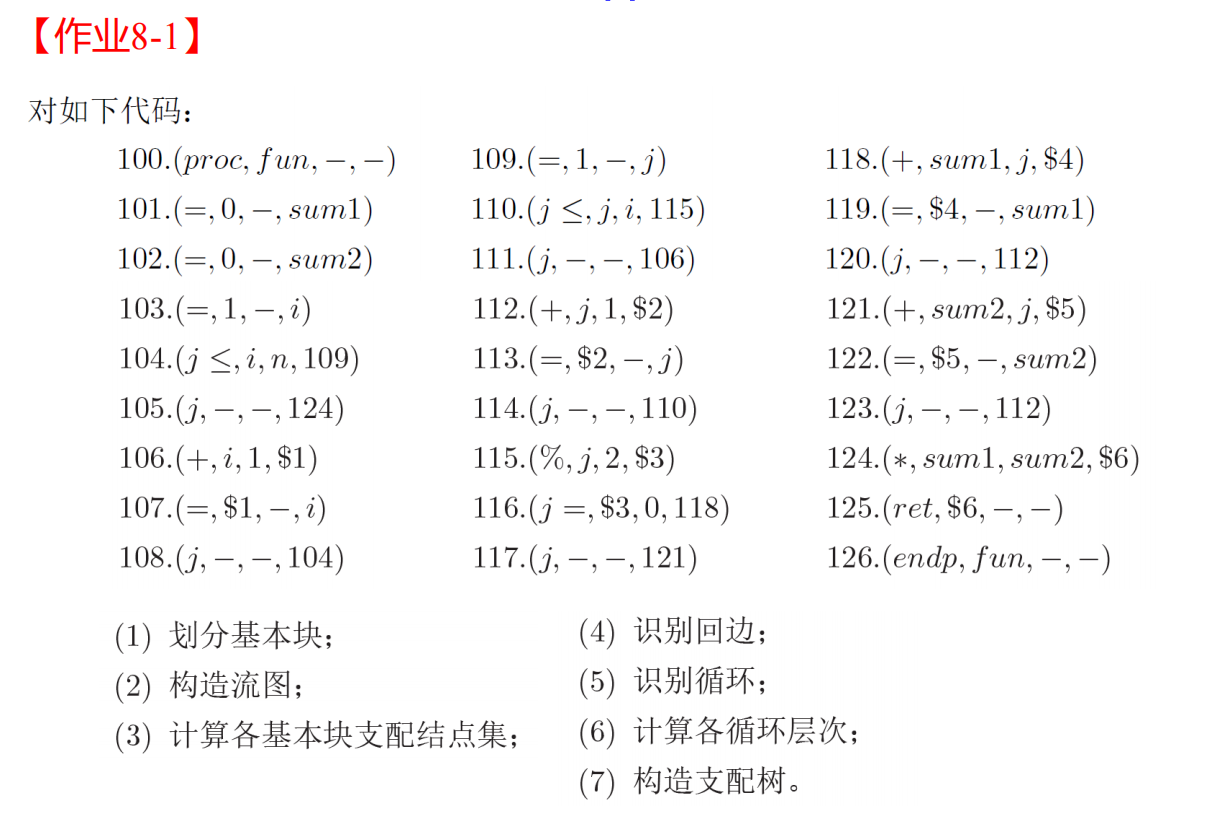
\includegraphics[width=0.9\linewidth]{imgs/8_1.png}
    \caption{作业 8.1——题目}
    \label{fig:8_1_prob}
\end{figure}
\subsubsection{解答}

求出基本块入口:

\begin{figure}[H]
    \centering
    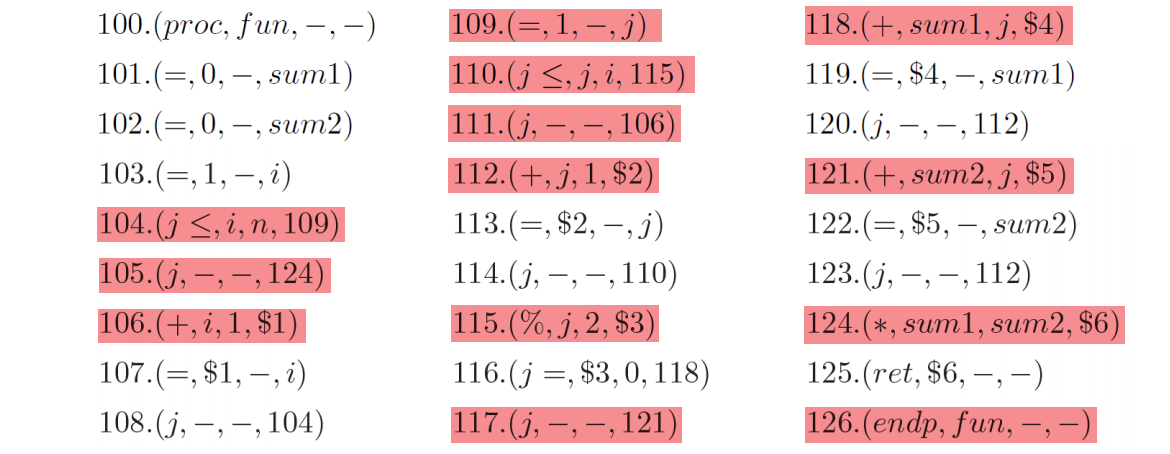
\includegraphics[width=0.9\linewidth]{imgs/8_1_1.png}
    \caption{作业 8.1——基本块入口}
    \label{fig:8_1_prob}
\end{figure}

划分基本块:

\begin{figure}[H]
    \centering
    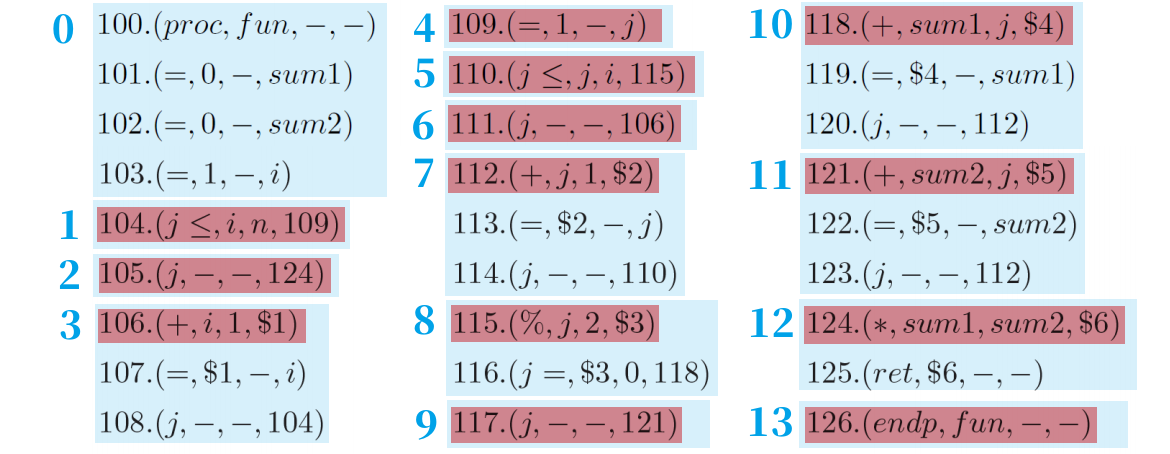
\includegraphics[width=0.9\linewidth]{imgs/8_1_2.png}
    \caption{作业 8.1——基本块}
    \label{fig:8_1_prob}
\end{figure}

构造流图:

\begin{center}
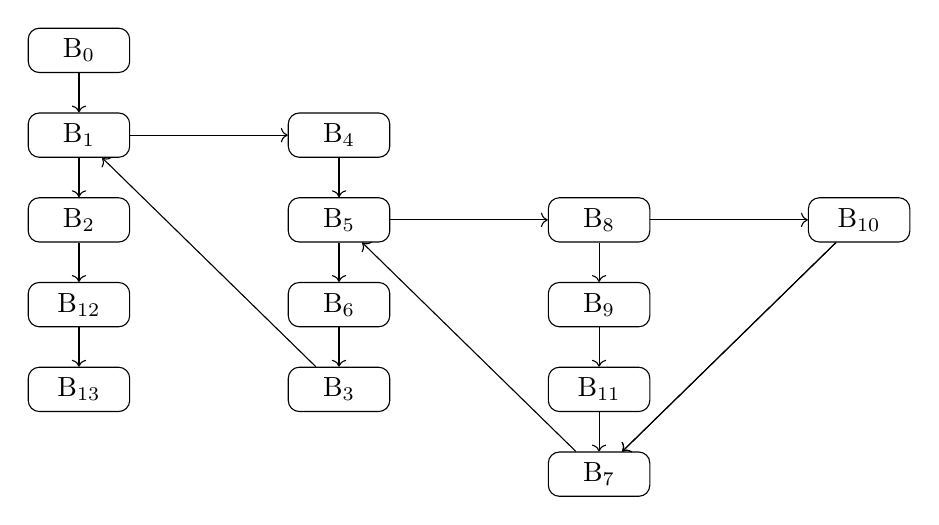
\begin{tikzpicture}[node distance=0.5cm, auto]
    \tikzstyle{block} = [rectangle, draw, fill=white!20, 
    text width=3em, text centered, rounded corners, minimum height=1.6em]

    \node [block] (B1) {$\text B_0$};
    \node [block, below=of B1] (B2) {$\text B_1$};
    \node [block, below=of B2] (B3) {$\text B_2$};
    \node [block, below=of B3] (B13) {$\text B_{12}$};
    \node [block, below=of B13] (B14) {$\text B_{13}$};

    \node [block, right=2cm of B2] (B5) {$\text B_4$};
    \node [block, below=of B5] (B6) {$\text B_5$};
    \node [block, below=of B6] (B7) {$\text B_6$};
    \node [block, below=of B7] (B4) {$\text B_3$};

    \node [block, right=2cm of B6] (B9) {$\text B_8$};
    \node [block, below=of B9] (B10) {$\text B_9$};
    \node [block, below=of B10] (B12) {$\text B_{11}$};
    \node [block, below=of B12] (B8) {$\text B_7$};

    \node [block, right=2cm of B9] (B11) {$\text B_{10}$};

    \draw [->] (B1) -- (B2);
    \draw [->] (B2) -- (B3);
    \draw [->] (B3) -- (B13);
    \draw [->] (B13) -- (B14);

    \draw [->] (B2) -- (B5);
    \draw [->] (B5) -- (B6);
    \draw [->] (B6) -- (B7);
    \draw [->] (B7) -- (B4);

    \draw [->] (B6) -- (B9);
    \draw [->] (B9) -- (B10);
    \draw [->] (B10) -- (B12);
    \draw [->] (B12) -- (B8);

    \draw [->] (B9) -- (B11);
    \draw [->] (B11) -- (B8);

    \draw [->] (B4) -- (B2);
    \draw [->] (B8) -- (B6);
    \draw [->] (B11) -- (B8);
\end{tikzpicture}
\end{center}

\subsection{作业8.2}
\subsubsection{题目描述}
\begin{figure}[H]
    \centering
    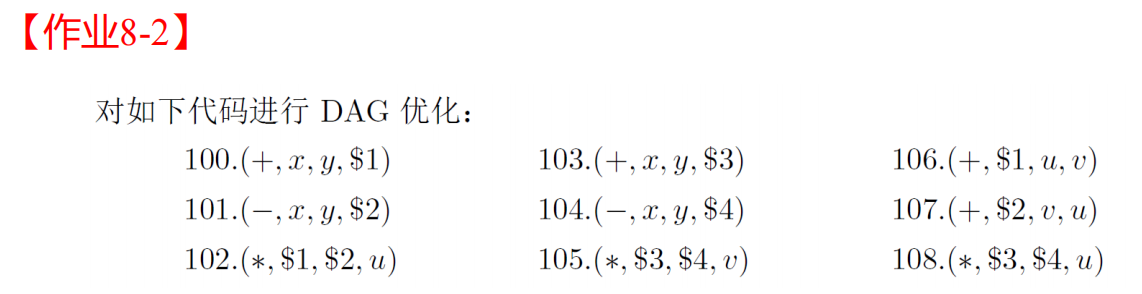
\includegraphics[width=0.9\linewidth]{imgs/8_2.png}
    \caption{作业 8.2——题目}
    \label{fig:8_2_prob}
\end{figure}
\subsubsection{解答}

使用 DAG 优化:

\begin{table}[H]
    \centering
    \begin{tabular}{c|c}
        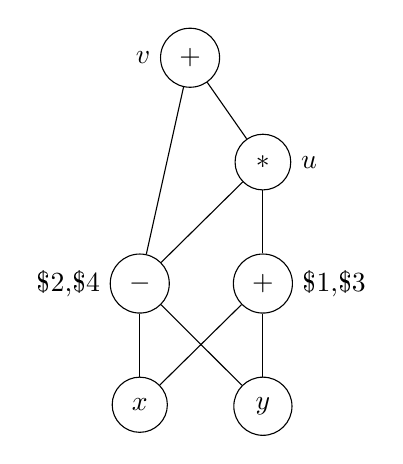
\begin{tikzpicture}[node distance=0.8cm, auto, baseline=(current bounding box.center)]
    \tikzstyle{block} = [circle, draw, fill=white!20, 
    text width=1em, text centered, rounded corners, minimum height=1em]

    \node [block, label={left:$v$}] (v) {$+$};
    \node [block, below right=0.8cm and 0.4cm of v, label={right:$u$}] (u) {$*$};
    \node [block, below=of u, label={right:\$1,\$3}] (plus) {$+$};
    \node [block, left=of plus, label={left:\$2,\$4}] (minus) {$-$};
    \node [block, below=of minus] (x) {$x$};
    \node [block, below=of plus] (y) {$y$};

    \draw [-] (v) -- node[auto] {} (u);
    \draw [-] (v) -- node[auto] {} (minus);
    \draw [-] (u) -- node[auto] {} (plus);
    \draw [-] (u) -- node[auto] {} (minus);
    \draw [-] (x) -- node[auto] {} (plus);
    \draw [-] (y) -- node[auto] {} (plus);
    \draw [-] (y) -- node[auto] {} (minus);
    \draw [-] (x) -- node[auto] {} (minus);
\end{tikzpicture}
        &
            \begin{tabular}{ll}
              100. & $(+,x,y,\$1)$ \\
              101. & $(=,\$1,-,\$3)$ \\
              102. & $(-,x,y,\$2)$ \\
              103. & $(=,\$2,-,\$4)$ \\
              104. & $(*,\$1,\$2,u)$ \\
              105. & $(+,\$1,u,v)$ \\
            \end{tabular}
        \\
    \end{tabular}
\end{table}


\newpage
	% 代码分析:模块功能、涉及到的类、类关系、数据结构及关键代码等;
	% 任务要求,设计任务要求;
	% 设计:详细的设计方案,相关的数据结构、算法描述,可采用伪代码等形式化描述
	% 实现:修改哪些类、如何修改、为什么修改等;
	% 测试:测试用例,测试结果及结果分析,测试运行界面等;
	% 调试:调试方法,遇到的问题及解决方案等;
	% 结论与展望:完成的主要工作、收获、进一步的工作,建议、体会、心得等;

\section{作业9}
\subsection{题目描述}
\begin{figure}[H]
    \centering
    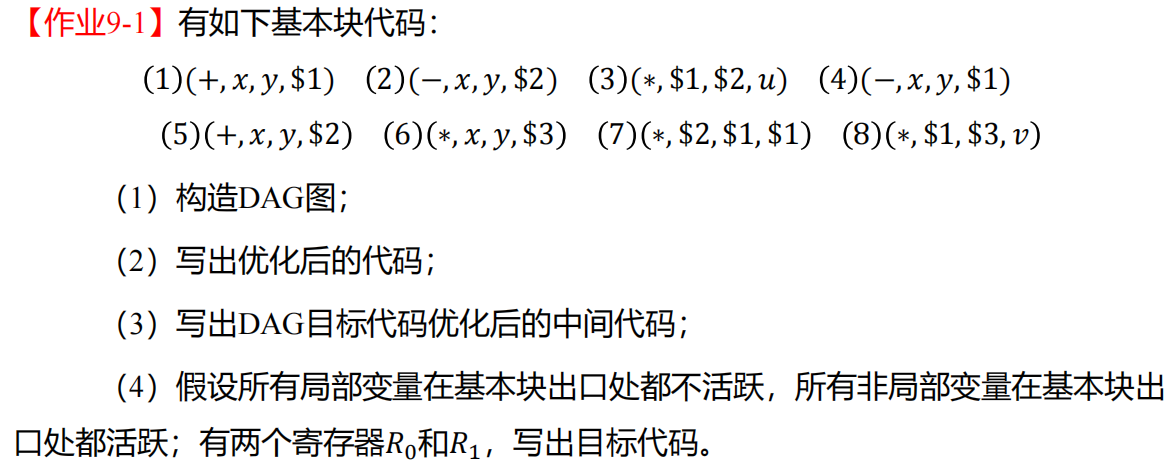
\includegraphics[width=0.9\linewidth]{imgs/9_1.png}
    \caption{作业 9.1——题目}
    \label{fig:9_1_prob}
\end{figure}
\subsection{解答}
\paragraph{构造 DAG 图、写出优化后的代码} 注意到两次计算 $x+y$ 与 $x-y$,分别赋给 \$1、 \$2 与 \$2、 \$1,可以重排 DAG 节点,同时不难对照 DAG 图写出代码:


\begin{table}[H]
    \centering
    \begin{tabular}{cc}
    \centering
    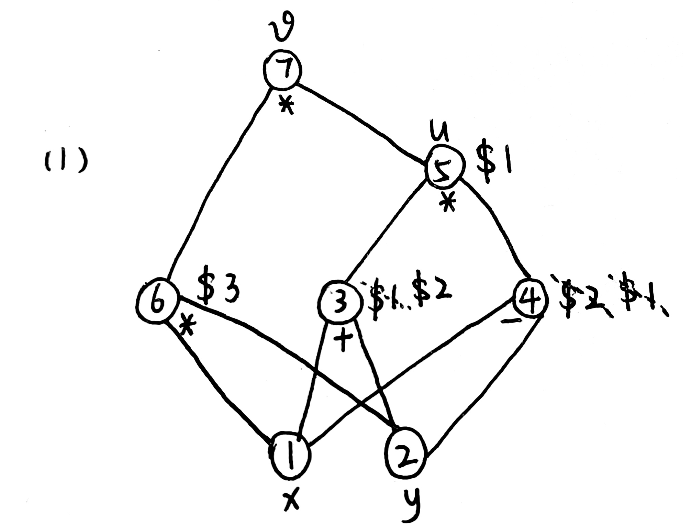
\includegraphics[width=0.4\linewidth]{imgs/9_1_1.png}
    & 
\begin{tabular}{rl}
(1) & $(+, x, y, \$1)$ \\
(2) & $(-, x, y, \$2)$ \\
(3) & $(*, \$1, \$2, u)$ \\
(4) & $(*, x, y, \$3)$ \\
(5) & $(*, u, \$3, v)$
\end{tabular}
\\
    \end{tabular}
\end{table}

\paragraph{写出 DAG 目标代码优化后的中间代码} 可以写出:

\begin{tabular}{rl}
(1) & $(*, x, y, \$3)$ \\
(2) & $(+, x, y, \$2)$ \\
(3) & $(-, x, y, \$\$1)$ \\
(4) & $(*, \$2, \$\$1, u)$ \\
(5) & $(*, \$3, u, v)$
\end{tabular}

\paragraph{写出目标代码} 可以写出:

\begin{table}[H]
\begin{tabular}{rll}
(1) &\quad$(*, x, y, \$3)$& \quad \text{\texttt{MOV R0 [ebp-$\hat \delta_x$]}} \\
  && \quad \text{\texttt{IMUL R0 [ebp-$\hat \delta_y$]}} \\
(2) &\quad$(+, x, y, \$2)$& \quad \text{\texttt{MOV R1 [ebp-$\hat \delta_x$]}} \\
  && \quad \text{\texttt{ADD R1 [ebp-$\hat \delta_y$]}} \\
(3) &\quad$(-, x, y, \$\$1)$& \quad \text{\texttt{MOV [ebp-$\hat \delta_{\$3}$] R0}} \\
  && \quad \text{\texttt{MOV R0 [ebp-$\hat \delta_{x}$]}} \\
  && \quad \text{\texttt{SUB R0 [ebp-$\hat \delta_{y}$]}} \\
(4) &\quad$(*, \$2, \$\$1, u)$& \quad \text{\texttt{IMUL R0 R1}} \\
(5) &\quad$(*, \$3, u, v)$& \quad \text{\texttt{MOV [ebp-$\hat \delta_{\$3}$] R1}} \\
  && \quad \text{\texttt{MOV [ebp-$\hat \delta_{u}$] R1}} \\
  && \quad \text{\texttt{IMUL R0 R1}} \\
  && \quad \text{\texttt{MOV [ebp-$\hat \delta_{v}$] R0}}
\end{tabular}
\end{table}


\end{document} 


